%%
%% Chapter
%%
\chapter{Markov Processes and Master Equations}

This chapter is devoted
to the introduction of some mathematical concepts, which allow the
correct treatment of time--dependent probabilistic phenomena. 
Such processes occur in many branches of physics. A typical example,
is for instance, the dynamics of the velocity field in a turbulent fluid.
We will introduce stochastic processes as time dependent stochastic 
variables and we will 
learn how the dynamics of a particular class of stochastic 
processes, the so--called Markov processes  is described 
with the help of differential Chapman--Kolmogorov equations. 
These concepts will be applied
in the next chapters to typical examples from statistical physics.

\section{Stochastic Processes}
We have already learned in Chap. 2 that once a stochastic variable 
$X$ has been defined it is possible to define other stochastic 
variables, say $Y$, as functions of $X$ by some mapping $f$. In 
particular, the quantity $Y$ may be a function of an additional
time variable $t$, i.e.,
\begin{equation*}
Y(t) = f(X,t).
\end{equation*}
Sloppy speaking, such a quantity $Y(t)$ is called a {\em stochastic
processes}. If we insert for $X$ one of its possible values $x$
we obtain an ordinary function
\begin{equation*}
y(t) = f(x,t),
\end{equation*}
which is a {\em realization} of the stochastic process
\cite{VAN_KAMPEN}. It is 
customary in statistical physics to regard the stochastic process 
as an {\em ensemble} of such realizations.

It follows immediately from the random variable transformation 
theorem that the probability density for $Y(t)$ to take the value
$y$ at time $t$ is given by
\begin{equation*}
P_1(y,t) = \int dx  \delta(y-f(x,t)) P(x)
\end{equation*}
and, accordingly, the joint probability density that $Y$ has the
value $y_1$ at time $t_1$, the value $y_2$ at time $t_2$, 
$\ldots$, and the value $y_n$ at time $t_n$ is given by
\begin{eqnarray*}
\lefteqn{P_n(y_1,t_1;y_2,t_2; \ldots, y_n,t_n)} \\
&& = \int dx \delta(y_1-f(x,t_1))\delta(y_2-f(x,t_2)) \cdots 
   \delta(y_n-f(x,t_n))  P(x).
\end{eqnarray*}
In such a way an infinite hierarchy of joint probability densities
$P_n$ $(n=1,2,\ldots)$ is defined, which allows the evaluation of 
expectation values like
\begin{eqnarray*}
\lefteqn{<Y(t_1) Y(t_2) \cdots Y(t_n)>} \\
&& = \int dy_1 \int dy_2 \cdots \int dy_n 
        y_1 y_2 \cdots y_n P_n(y_1,t_1;y_2,t_2; \ldots, y_n,t_n).
\end{eqnarray*}
It has been shown by Kolmogorov (\cite{VAN_KAMPEN}) that the 
hierarchy of joint probability densities introduced above 
completely specifies
a stochastic process if the following four consistency conditions 
are satisfied \\
(i) $P_n \ge 0$; \\
(ii) $P_n$ is a symmetric function of the pairs $(y_1,t_1)$, 
$\ldots$, $(y_n,t_n)$; \\
(iii) $\int dy_n P_n(y_1,t_1; \ldots , y_n,t_n) =
     P_{n-1}(y_1,t_1; \ldots ; y_{n-1},t_{n-1})$; \\
(iv) $\int dy_1 P(y_1,t_1) =1$.

Thus, the hierarchy of joint probability densities constitutes an 
alternative way to define stochastic processes. 
With increasing $n$ the description of the stochastic process gets
more precise. It is important to 
make the following remarks.  The condition (iii) implies that each 
density $P_n$ includes the knowledge of all previous densities
$P_k$ with $k<n$. Furthermore, the density $P_n$ does have the 
following property if two time arguments are identical
\begin{equation*}
P_n(x,t;y_1,t;y_2,t_2; \ldots ; y_{n-1},t_{n-1}) = 
P_{n-1}(x,t;y_2,t_2; \ldots ; y_{n-1},t_{n-1})
\delta(x-y_1).
\end{equation*}
The hierarchy of probability densities is also the starting point 
for the classification of stochastic processes. A stochastic 
process is said to be purely random if events at different times 
are not correlated. In this case the joint probability density 
factorizes, i.e. we have
\begin{eqnarray*}
P_2(y_1,t_1;y_2,t_2) &=& P_1(y_1,t_1) P_1(y_2,t_2) \\
P_3(y_1,t_1;y_2,t_2;y_3,t_3) &=& P_1(y_1,t_1) P_1(y_2,t_2)P_1(y_3,t_3) 
\\
\text{and so on.} &&
\end{eqnarray*}
This means that the value of $Y$ at time $t$ is completely 
independent of its values in the past and in the future. An even
more special case occurs when the $P_1(y_i,t_i)$ are independent 
of $t_i$. In this case the same probability law governs the 
process for all times. Such processes are called
{\em Bernoulli trials} (\cite{gardiner}). In the next section we 
will introduce the next most simple class, the {\em Markov processes},
in which the knowledge of only the presents determines the future.


\section{Markov Processes}
In order to define the class of stochastic processes, which will be 
of central importance in the forthcoming theoretical discussions 
and in the examples of the next chapters, we will formulate
the {\em Markov assumption}. This assumption is formulated in 
terms of conditional probability densities which we 
will denote by
$T_n(x,t|y_1,t_1;y_2,t_2; \ldots, y_n,t_n)$. This quantity gives 
the probability that the stochastic process takes the value $x$ at 
time $t$ given that it had the value $y_1$ at time $t_1$, $y_2$
at time $t_2$, $\ldots$, $y_n$ at time $t_n$, where we assume that
$t_1< \cdots <t_n < t$.  The conditional probability density has 
the following properties \\
(i) $T_n \ge 0$, \\
(ii) $\int dx T_n = 1$,  \\
(iii) $T_n(x,t|y_1,t;y_2,t_2; \ldots, y_n,t_n) = \delta(x-y_1)$.\\
As we already know the joint probability density $P_n$ can be 
expressed with the help of Bayes' theorem through the conditional 
probability density $T_{n-1}$ as
\begin{eqnarray*}
\lefteqn{P_n(x,t;y_1,t_1;y_2,t_2; \ldots, y_{n-1},t_{n-1})} \\
&& = P_{n-1}(y_1,t_1;y_2,t_2; \ldots, y_{n-1},t_{n-1})
T_{n-1}(x,t|y_1,t_1;y_2,t_2; \ldots, y_{n-1},t_{n-1}).
\end{eqnarray*}
Now we are in the position to define the class of Markov 
processes. Let $t_1< \cdots <t_n < t_{n+1}$ be an ordered sequence 
of times. A Markov process is defined through the following 
condition for the conditional probability density of the
stochastic process
\begin{equation*}
T_{n}(y_{n+1},t_{n+1}|y_1,t;y_2,t_2; \ldots, y_{n},t_{n})
= T_{1}(y_{n+1},t_{n+1}|y_{n},t_{n}).
\end{equation*}
In other words, the conditional probability density at $t_{n+1}$
given the value of $y_n$ at time $t_n$ is uniquely determined and 
is not affected by any value of $y$ at earlier times. Thus, the
conditional probability density is determined completely by the 
knowledge of the most recent condition.
The above definition implies that for a Markov process all
$T_n$ with $n \ge 1$ can be determined from the
conditional probability density $T_1$, which will also be called
the one step 
transition probability density. As an immediate consequence a Markov 
processes is completely characterized by the knowledge of the
one step transition probability and by the probability density
$P_1$. With the help of these two functions we can reconstruct the 
whole hierarchy of probability densities. For example, we
have
\begin{eqnarray}
\label{P3}
P_3(y_1,t_1;y_2,t_2;y_3,t_3) &=& 
      P_2(y_1,t_1;y_2,t_2) T_2(y_3,t_3|y_1,t_1;y_2,t_2)   
         \nonumber \\
    & = & T_1(y_3,t_3|y_2,t_2) T_1(y_2,t_2|y_1,t_1)
           P_1(y_1,t_1).
\end{eqnarray}
Integrating the above equation (\ref{P3}) over $y_2$ we obtain 
\begin{equation}
P_2(y_1,t_1;y_3,t_3) = P_1(y_1,t_1) 
       \int dy_2 T_1(y_3,t_3|y_2,t_2) T_1(y_2,t_2|y_1,t_1).
\end{equation}
Dividing both sides by $P_1(y_1,t_1)$ we obtain an identity which 
must be obeyed by the transition probability of any Markov process
\begin{equation}
\label{CHAPMAN_KOLMOGOROV}
T_1(y_3,t_3|y_1,t_1) =  
       \int dy_2 T_1(y_3,t_3|y_2,t_2) T_1(y_2,t_2|y_1,t_1).
\end{equation}
The above identity is called the {\em Chapman--Komogorov 
equation}. It has a simple interpretation. The transition 
probability between two states $y_1$ and $y_3$ with $t_1 <t_3$
corresponds to the product of the transition probability between 
the initial state and some intermediate state and the transition 
between this intermediate state and the final state integrated
over all intermediate states.

As we already noted the functions $P_1$ and $T_1$ uniquely define 
a Markov process. However, these two functions are not arbitrary.
They must satisfy the Chapman--Kolmogorov equation and the obvious
consistency condition
\begin{equation}
\label{CONSISTENCY}
P_1(y_2,t_2) =  
       \int dy_1  T_1(y_2,t_2|y_1,t_1) P_1(y_1,t_1).
\end{equation}
For the sake of a compact notation we will write now $P=P_1$ and 
$T=T_1$.


\section{The Differential Chapman--Kolmogorov Equation}
We now derive a differential  form of the Chapman--Kolmogorov 
equation which is more practical for physical applications.
We will proceed in two steps. First, we introduce the concept
of generator of a stochastic process. Second, we will construct
with the help of the generator an equation of motion for the
transition probabilty density.

\subsection{The Generator of a Markov Process}
We consider the time evolution of the expectation value
of  a function $f(y)$.
Thus,
\begin{eqnarray*}
\frac{\partial}{\partial t} \langle f(y) \rangle &=&
 \frac{\partial}{\partial t} 
    \left\{  \int dy f(y) P(y,t)  \right\}  \\
 &= & \lim_{\Delta t \rightarrow 0} \frac{1}{\Delta t}
       \left\{  \int dy f(y) \left[P(y,t+\Delta t) - P(y,t) \right]  
       \right\}.
\end{eqnarray*}
Making use of the consistency condition (\ref{CONSISTENCY}) 
in the first term 
on the right--hand side of the above equation we obtain
\begin{equation*}
\frac{\partial}{\partial t} \langle f(y) \rangle =
   \lim_{\Delta t \rightarrow 0} \frac{1}{\Delta t}
    \left\{  \int dy \int dy' f(y) T(y,t+\Delta t|y',t) P(y',t) 
         - \int dy f(y) P(y,t) 
       \right\}.
\end{equation*}
We rename the integration variables in the positive 
term of the right--hand side of the above equation ($y \rightarrow y'$,
$y' \rightarrow y$) to obtain
\begin{equation*}
\frac{\partial}{\partial t} \langle f(y) \rangle =
   \lim_{\Delta t \rightarrow 0} \frac{1}{\Delta t}
    \left\{  \int dy  \int dy' \left[ f(y') T(y',t+\Delta t|y,t) 
         - \delta(y-y') f(y') \right] P(y,t) 
       \right\},
\end{equation*}
which we can also write as
\begin{equation*}
\frac{\partial}{\partial t} \langle f(y) \rangle =
\int dy P(y,t) \lim_{\Delta t \rightarrow 0} \frac{1}{\Delta t}
\left\{ \int dy' \left[ f(y') T(y',t+\Delta t|y,t) 
         - \delta(y-y') f(y') \right].
\right\}
\end{equation*}
At this point it is convenient to introduce the infinitesimal 
generator of a Markov process ${\cal{A}}$ as
\begin{equation}
\label{DEF_GENERATOR}
{\cal{A}}(t) f(x) = \lim_{\Delta t \rightarrow 0}
    \frac{1}{\Delta t} 
    \left[\int dy f(y)T(y,t+\Delta t|x,t) - f(x)  \right].
\end{equation}
$f(y)$ is some measurable function for which the above 
limit exists. Evidently ${\cal{A}}$ is a linear operator, which 
can be determined from the transition probability density. 
When the operator ${\cal{A}}$ operates on $f$ it describes the
change of the expectation value of $f$ in an infinitesimal time 
step. As a consequence of the Chapman--Kolmogorov equation each time 
step $t-t_1$ can be decomposed into a sequence of smaller time 
steps. So it is plausible to characterize the Markov
process by regarding infinitesimal time steps. 
The importance of the generator ${\cal{A}}$ lies in the fact
that together with some initial condition $P(x,t=0)$ it specifies
uniquely the Markov process.
The time evolution equation for the expectation value can be written 
in the compact and suggestive form
\begin{equation}
\label{EQ_EXPECTATION}
\frac{\partial}{\partial t} \langle f \rangle = 
\langle {\cal{A}} f \rangle.
\end{equation}


\subsection{The Differential Chapman--Kolmogorov Equation}
With the help of the generator we derive an equation of motion for
the transition probability $T$.
Multiplying equation (\ref{DEF_GENERATOR}) 
with $T(x,t|x',t')$ ($t'<t$) and 
integrating over $x$ we obtain
\begin{eqnarray*}
\lefteqn{\int dx \left[ {\cal{A}}(t) f(x) \right] T(x,t|x',t')} \\
&& = \lim_{\Delta t \rightarrow 0}
    \frac{1}{\Delta t} 
    \left[\int dy f(y)T(y,t+\Delta t|x',t') - 
        \int dx f(x) T(x,t|x',t')  \right],
\end{eqnarray*}
where we made use of the Chapman--Kolmogorov equation.
We now rename the variable $y$ on the right--hand side of the above 
equation and call it $x$ and perform the limit $\Delta t \rightarrow 
0$
\begin{equation}
\label{KOL_FORWARD_0}
\int dx \left[ {\cal{A}}(t) f(x) \right] T(x,t|x',t') =
  \int dx f(x) \frac{\partial}{\partial t} T(x,t|x',t').
\end{equation}
It is convenient to introduce the adjoint operator ${\cal{A}}^{\dagger}$
to the generator ${\cal{A}}$ according to the following definition
\begin{equation}
\label{ADJOINT}
\int dx \left[ {\cal{A}}(t) f(x) \right] T(x,t|x',t') \equiv
\int dx f(x) \left[ {\cal{A}}^{\dagger}(t)  T(x,t|x',t') \right].
\end{equation}
We will see in the next sections how the adjoint operator is
explicitely constructed.
Inserting Eq. (\ref{ADJOINT}) into Eq. (\ref{KOL_FORWARD_0})
and considering that (\ref{ADJOINT}) holds for any 
function $f(x)$ we conclude that the equation of motion for the 
transition probability is given by
\begin{equation}
\label{KOL_FORWARD}
\frac{\partial}{\partial t} T(x,t|x',t') =
{\cal{A}}^{\dagger}(t) T(x,t|x',t').
\end{equation}
We will call the above equation the {\em differential 
Chapman--Kolmogorov equation}. The differential 
Chapman--Kolmogorov equation is the central equation of this 
chapter. Together with some initial probability distribution it 
defines completely a Markov process. With its help it is possible
to compute time--dependent expectation values and multi--time 
correlation functions. Because of its importance, it is sometimes
named the {\em master equation} in the physical literature.


Let us end this subsection with an overview of this chapter. In Fig. 
(\ref{F_CHAP$_OVERVIEW}) we have schematically summerized the theory
of stochastic processes.  Particular emphasis is given to Markov
processes
which will be at the center of the present and of the next chapters.
In the next section we will construct
the differential Chapman--Komogorov equation for deterministic Markov 
processes, for jump processes and for diffusion processes.
\begin{figure}
\label{F_CHAP$_OVERVIEW}
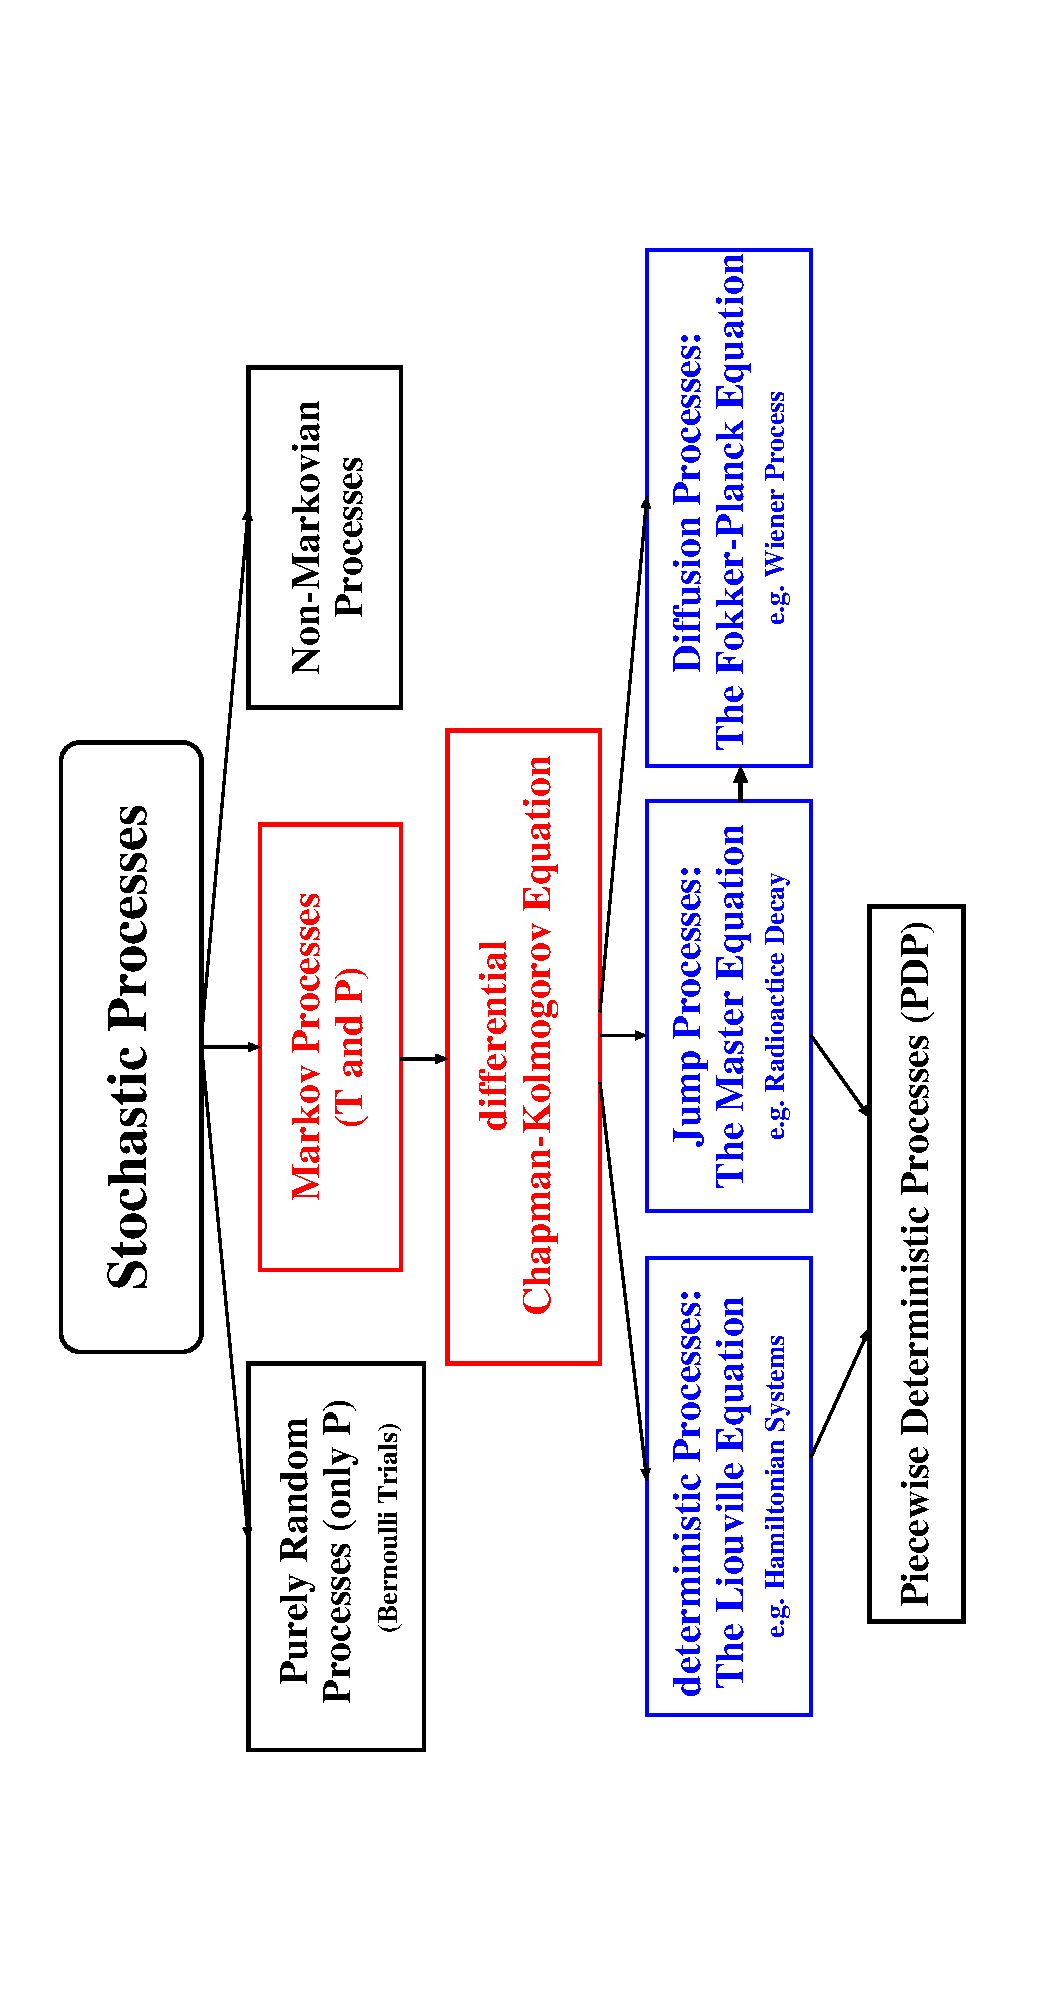
\includegraphics[width=10cm]{./Figures/f_chap4_overview.eps}
\caption{Overview of the theor of stochastic processes.}
\end{figure}

\section{The Liouville Equation}
Let us consider a physical system whose dynamics is described
by a system of ordinary differential equations of first order
\begin{equation}
\label{ORDINARY_DIFF}
\frac{d}{dt} x(t) = g(x(t)),
\end{equation}
where $g$ is a function $R^d \rightarrow R^d$. 
It is clear that Hamiltonian systems belong to this class 
(\cite{ARNOLD}). The initial 
condition is
\begin{equation*}
x(0) = x \in R^d.
\end{equation*}
We denote the unique solution of this equation by $\phi(t,x)$,
where the $x$ stresses the dependence on the initial condition.

If $f:R^d \rightarrow R^d$ is a continuous differentiable function
then it follows from Eq. (\ref{ORDINARY_DIFF}) 
\begin{equation}\label{COORDINATE_FREE}
\frac{d}{dt} f(x(t)) = \sum_i \frac{\partial f}{\partial x_i}
          (x(t)) g^i(x(t)),
\end{equation}
where $g^i$ denotes the $i$--th component of $g$. 


With the help of these formal preliminaries it is easy to 
construct the generator of a deterministic Markov process.
Obviously we have for the expectation value
\begin{equation*}
Ef(x(t)) = f(\phi(x,t)),
\end{equation*}
where the symbol $E$ denotes the expectation value.

Inserting the above expectation value into the definition of a 
generator (\ref{DEF_GENERATOR}) we immediately obtain
\begin{eqnarray*}
{\cal{A}}_L(t) f & = & \lim_{t\rightarrow 0} \frac{1}{t}
                        \left[ Ef(x(t)) - f(x)\right] \\
             & = & \lim_{t\rightarrow 0} \frac{1}{t}
                        \left[ f(\phi(x,t)) - f(\phi(0,x))\right] \\
              & = & \frac{d}{dt} f(x) ,
\end{eqnarray*}
and finally, using Eq. (\ref{COORDINATE_FREE}),
\begin{equation*}
{\cal{A}}_L(t) f = \sum_i \frac{\partial f}{\partial x_i}(x) g^i(x).
\end{equation*}


Having determined the generator it is now straightforward to 
evaluate the corresponding differential Chapman--Kolmogorov 
equation. To this end we only 
have to determine the operator which is adjoint to
${\cal{A}}_L$ by partial integration. It is evident that we have
\begin{eqnarray}
\label{GEN_DET0}
\int dx \left[{\cal{A}}_L f(x) \right]h(x) &=&
          \sum_i \int dx \left[g^i 
           \frac{\partial f}{\partial x_i} \right] h(x) \nonumber \\
     & = & -\sum_i f \frac{\partial}{\partial x_i} g^i h(x).      
\end{eqnarray}
Since Eq. (\ref{GEN_DET0}) holds for any function $h(x)$
\begin{equation}
\label{GEN_DET_A}
{\cal{A}}_L^{\dagger} h(x) = -\sum_i \frac{\partial}{\partial x_i}
    \left(g_i h(x) \right).
\end{equation}
Inserting (\ref{GEN_DET_A}) into the differential Chapman--Kolmogorov 
equation
(\ref{KOL_FORWARD}) 
leads to the master equation for a deterministic Markov process
\begin{equation}
\frac{\partial}{\partial t} T(x,t|x',t') =
 - \sum_i \frac{\partial}{\partial x_i}
     \left(g_i(x)T(x,t|x',t')  \right).
\end{equation}
In statistical physics the above equation is called the Liouville 
equation.
 
The Liouville equation is the starting point for the microscopic 
description of matter for classical as well as for quantum 
mechanical systems. It is one of the fundamental equations of 
statistical physics. 

\subsection{Example: Classical Statistical Mechanics}
In order to give an example of the occurrence
of the Liouville equation we consider a closed classical system
with $N$ degrees of freedom, e.g., $N$ particles in a 
three--dimensional box. We know from classical mechanics, that the 
state  of such a system is completely specified by the set of $6N$
independent variables $\vec{p}^N=(\vec{p}_1, \ldots, \vec{p}_N)$ 
and $\vec{q}^N=(\vec{q}_1, \ldots, \vec{q}_N)$, where $\vec{p}_i$
and $\vec{q}_i$ denote the momentum and the position of the 
$i$--th particle. 

If the system is Hamiltonian (\cite{ARNOLD}), 
i.e., if we can define a Hamiltonian
$H(\vec{p}^N,\vec{q}^N)$, then the time evolution of the momentum 
and of the position of the particles is given by Hamilton's 
equations of motion
\begin{eqnarray*}
\frac{d}{dt} \vec{p}_i &=& - \frac{\partial H}{\partial \vec{q}_i} 
             \\
\frac{d}{dt} \vec{q}_i &=&  \frac{\partial H}{\partial \vec{p}_i} 
.
\end{eqnarray*}

In a real physical system it is not possible to specify exactly 
the state of the system. There is always some uncertainty in the 
initial conditions. Therefore, we regard $(\vec{p}^N,\vec{q}^N)$
as a stochastic variable which is initially distributed according 
to the joint probability density $P^N(\vec{p}^N,\vec{q}^N,0)$. 
The dynamics of this probability distribution
is described by the following 
Liouville equation
\begin{equation*}
\frac{\partial}{\partial t} P^N =  {\cal{A}}_L^{\dagger} P^N,
\end{equation*}
where
\begin{equation*}
{\cal{A}}_L^{\dagger} = -\sum_{i=1}^N \left( 
      \frac{\partial H}{\partial \vec{p}_i} 
            \cdot \frac{\partial}{\partial \vec{q}_i} 
         - \frac{\partial H}{\partial \vec{q}_i} 
             \cdot \frac{\partial}{\partial \vec{p}_i}.
      \right)
\end{equation*}
The Liouville equation is often written in the following form
\begin{equation*}
i \frac{\partial}{\partial t} P^N(\vec{p}^N,\vec{q}^N,t) =  
  {\cal{L}} P^N(\vec{p}^N,\vec{q}^N,t),
\end{equation*}
where
\begin{equation*}
{\cal{L}} =  i {\cal{A}}_L^{\dagger}.
\end{equation*}
The operator ${\cal{L}}$ is called the Liouville operator.
If the probability disribution at time $t=0$ is known the above 
Liouville equation may be integrated formally  
to find the probability density
at later times $t$
\begin{equation*}
P^N(\vec{p}^N,\vec{q}^N,t) = \exp(-i {\cal{L}}t)  
P^N(\vec{p}^N,\vec{q}^N,0).
\end{equation*}
The Liouville equation is the starting point for the evaluation of 
probability distributions in statistical mechanics. Extensive use 
of the Liouville equation is done in kinetic theory. From the 
Liouville equation it is possible to derive a hierarchy of 
equations for probability densities, the so--called 
BBGKY--hierarchy from which kinetic equations may be derived
(\cite{REICHL}).


\section{The Master Equation}
Let us now introduce jump processes (\cite{DAVIES,FELLER}).
We consider a system in a given state $x$.  
In order to characterize a jump process, i.e., a process
in which the system undergoes sudden discontinuous changes of its state,
we have to specify the probability for 
the system to remain in $x$ during the time interval $dt$ 
\begin{equation*}
(1-\lambda(x) dt)
\end{equation*}
and the probability that the system jumps from state $x$ to state
$x'$ during the time interval $dt$ 
\begin{equation*}
\lambda(x) Q(x',x) dt,
\end{equation*}
where
\begin{equation}
\label{NORM_Q}
\int dx' Q(x',x) =1.
\end{equation}
Then,
\begin{equation*}
Ef(x(dt+t)) = (1-\lambda(x)dt) f(x)
   + \lambda(x) dt \int dx'f(x') Q(x',x).
\end{equation*}
From the definition of the generator we obtain immediately the
generator of the jump process
\begin{equation}
\label{GEN_JUMP}
{\cal{A}}_M f(x) = \lambda(x) \int dx' \left( f(x') 
-f(x)\right)Q(x',x),
\end{equation}
where we made use of Eq. (\ref{NORM_Q}).
Again, in order to derive the Kolmogorov forward equation we have 
to construct the adjoint operator to ${\cal{A}}_M$.
We start from Eq. (\ref{KOL_FORWARD_0})  
\begin{equation}
\label{KOL_FORWARD_J0}
\int dx \left[ {\cal{A}}_M(t) f(x) \right] T(x,t|x',t') =
  \int dx f(x) \frac{\partial}{\partial t} T(x,t|x',t').
\end{equation}
and insert the generator (\ref{GEN_JUMP}) into the left--hand side 
of the above equation
\begin{eqnarray*}
\lefteqn{\int dx \left[ {\cal{A}}_M(t) f(x) \right] T(x,t|x',t')} 
\\
&=& \int dx \left[ \lambda(x)
       \int dx'' \left(f(x'') -f(x) \right) Q(x'',x) \right] T(x,t|x',t') 
       \\
& = & \int dx \int dx'' \lambda(x) f(x'') Q(x'',x) T(x,t|x',t') \\
& & - \int dx \int dx'' \lambda(x) f(x) Q(x'',x) T(x,t|x',t').
\end{eqnarray*}
By renaming $x \rightarrow x''$ and $x'' \rightarrow x$  in the first line of the
above equation we get
\begin{eqnarray}
\label{ADJOINT_JUMP}
\lefteqn{\int dx  f(x) \int dx'' \lambda(x'')  Q(x,x'') T(x'',t|x',t')}
     \nonumber \\
& & - \int dx f(x) \int dx'' \lambda(x)  Q(x'',x) T(x,t|x',t') \nonumber \\
& \equiv & \int dx f(x) \left[ {\cal{A}}_M^{\dagger}(x) 
          T(x,t|x',t')      \right]
\end{eqnarray}
From Eq. (\ref{KOL_FORWARD_J0}) and from Eq. (\ref{ADJOINT_JUMP}) 
we conclude that the differential Chapman--Kolmogorov equation 
of a jump process
reads
\begin{eqnarray} 
\label{KOL_FORWARD_J1}
\lefteqn{\frac{\partial}{\partial t} T(x,t|x',t') =} \nonumber \\ 
&& \int dx'' \lambda(x'') Q(x,x'') T(x'',t|x',t')
 - \int dx'' \lambda(x) Q(x'',x) T(x,t|x',t').
\end{eqnarray}
Because of Eq. (\ref{NORM_Q}) we can write the above equation also 
in the form
\begin{eqnarray} 
\label{KOL_FORWARD_J2}
\lefteqn{\frac{\partial}{\partial t} T(x,t|x',t') =} \nonumber \\ 
&& \int dx'' \lambda(x'') Q(x,x'') T(x'',t|x',t')
 - \lambda(x) T(x,t|x',t').
\end{eqnarray}
Usually the differential Chapman--Kolmogorov equation for a jump process is 
written in a more suggestive form. To this end we introduce the 
total transition rate pro time unit for a transition from state $x'$ 
into  state $x$ to occur
\begin{equation*}
w(x,x') = \lambda(x') Q(x,x')
\end{equation*}
and write the differential Chapman--Kolmogorov equation 
for a jump process in its final form
\begin{equation}
\label{MASTER_JUMP}
\frac{\partial}{\partial t} T(x,t|x',t') =
 \int dx'' \left( w(x,x'') T(x'',t|x',t')
 - w(x'',x) T(x,t|x',t') \right).
\end{equation}
The above equation is called the master equation. 
The name master equation appears for the first time in a paper by
Nordsieck, Lamb and Uhlenbeck (\cite{NORDSIECK}). 
It was chosen to denote an equation from which
all relevant equations and results can be derived. 

In the physical literature Eq. (\ref{MASTER_JUMP}) is written in 
the simplified form
\begin{equation}
\label{MASTER_JUMP_P}
\frac{\partial}{\partial t} P(x,t) =
 \int dx'' \left( w(x,x'') P(x'',t)
 - w(x'',x) P(x,t) \right).
\end{equation}
This equation has the following meaning (\cite{VAN_KAMPEN}). Take a 
time $t'$ and a state $x'$ and consider 
the solution of Eq. (\ref{MASTER_JUMP_P})
for $t \ge t'$ with the initial condition $P(x,t') = 
\delta(x-x')$. This solution is the conditional transition 
probability $T(x,t|x',t')$ of the Markov process for each choice
of $x'$ and $t'$. It is important to keep in mind that 
Eq. (\ref{MASTER_JUMP_P})
is always to be interpreted as an equation for $T$ and not for 
$P$.

In the above form the physical meaning of the master equation is 
also evident. The master equation is a balance equation for the
probability to find the system in some state. The first term in 
the master equation describes the gain of state due to transitions 
from the other states. The second term is the loss due to the 
transitions from the given state into the others. Evidently,
the term with $x=x'$ does not contribute to the integral.

If the state space of the stochastic process is discrete, i.e.
all integer numbers $n$,
the master equation for the time evolution of $P(n,t)$ will assume 
the following discrete form
\begin{equation}
\label{MASTER_JUMP_P_N}
\frac{\partial}{\partial t} P(n,t) =
 \sum_{n'} \left( w(n,n') P(n')
 - w(n',n) P(n,t) \right).
\end{equation}
We will discuss in the next section how the stochastic processes 
defined in terms of a master equation can be simulated 
numerically.


\section{Stochastic Simulation}
In principle there are two ways to treat numerically
stochastic processes which are defined in terms of master
equations. In the first approach one solves numerically the
master equation as a differential equation for the probability
density. Although this deterministic method is direct we will not consider it 
here for the following reason. It  turns out that the direct 
numerical solution of the master equation is not particularly 
efficient from a computational point of view. The second approach,
which we will introduce in this section relies upon the simulation 
of the underlying stochastic process. In other words one considers 
a particle and lets it jump from one state to another with certain 
given transition rates. Such a procedure is called the generation 
of a realization of the stochastic process. If a sufficiently 
great number of realizations has been generated the interesting 
statistical quantities can be evaluated as ensemble averages.

In fact the numerical performance of the direct approach gets 
worse compared to the stochastic simulation with increasing 
dimension of the system considered. We already met a similar 
situation, when we considered numerical algorithms for the 
computation of integrals. There the direct integration of 
multidimensional integrals turned out to be less efficient than 
the Monte--Carlo integration.

In order to formulate a stochastic simulation algorithm we 
consider for simplicity the master equation of a one--step 
process. Sometimes such processes are also called birth--and--death
processes. The range of such processes consists of all integers
$n$ and the matrix of the transition probabilities per unit time
allows only jumps between adjacent sites
\begin{equation*}
w(n',n) \neq 0 \;\;\; \text{for} \;\;\; n'=n \pm 1
\end{equation*}
and
\begin{equation*}
w(n',n) = 0 \;\;\; \text{otherwise}.
\end{equation*}
Exploiting the above structure we can write the master equation 
for the discrete one--dimensional process (\ref{MASTER_JUMP_P_N})
\begin{eqnarray*}
\dot{P}(n,t) &=& w(n,n+1)P(n+1,t) + w(n,n-1)P(n-1,t) \\
       && -w(n+1,n)P(n,t) -w(n-1,n)P(n).
\end{eqnarray*}
Now it is convenient to introduce the following notation
\begin{eqnarray*}
r(n+1) \equiv w(n,n+1) \\
g(n-1) \equiv w(n,n-1),
\end{eqnarray*}
so that the master equation for a general one--step process 
may be written in the following 
suggestive form
\begin{equation}
\label{MASTER_ONE_STEP}
\dot{P}(n,t) = r(n+1)P(n+1,t) + g(n-1)P(n-1,t)
        -[r(n)+ g(n)]P(n,t).
\end{equation}

Let us now assume that at time $t$ the particle is in state
$n$. The total transition rate to leave this state, i.e. to jump 
out of this state either to state $n+1$ or to state $n-1$, is 
given by
\begin{equation}
\label{TOTAL_RATE_ONE_JUMP}
\lambda(n) = r(n) + g(n).
\end{equation}
As we already know  the quantity $\lambda(n) dt$ is the 
probability that the next jump occurs within the infinitesimal 
time step $dt$. Accordingly the probability that the next jump 
occurs after $(N+1)$ time steps $dt$ is given by
\begin{equation*}
q=[1-\lambda(n)dt]^N \lambda(n)dt,
\end{equation*}
where $[1-\lambda(n)dt]^N$ denotes the probability that no jump
occurs during the first $N$ steps. We now write $(N+1)dt =t$, so 
that we have
\begin{equation*}
q= \left( 1 - \frac{\lambda(n) t}{N+1}\right)^N \lambda(n) dt.
\end{equation*}
We now perform the limit $dt \rightarrow 0$ for fixed $t$. This 
limit implies, of course, $N \rightarrow \infty$ and hence the 
probability that a jump occurs after time $t$ is given by
\begin{equation*}
q= \lambda \exp(-\lambda t) dt = f(t) dt.
\end{equation*}
The waiting time distribution for the time of the next jump is an
exponential distribution.
It is now clear what we have to do in order to determine the time 
of the next jump in the stochastic simulation.  
We simply have to draw random times $\tau$, 
which are distributed according to the density $f(t)$. Since $f(t)$
is an exponential distribution, these random times can easily be 
drawn with the help of the inversion method
\begin{equation}
\label{TAU_ONE_STEP}
\tau = - \frac{1}{\lambda(n)} \log(\xi),
\end{equation}
where $\xi$ is a uniformly distributed random number on the 
interval $[0,1)$. 

Having determined the stochastic time of the
next jump we still have to decide which transition actually takes 
place. We have only two possibilities: In case of a jump the 
particle can reach the state $(n-1)$ with probability
\begin{equation*}
y_1 = \frac{r(n)}{\lambda(n)}
\end{equation*}
or the state  $(n+1)$ with probability
\begin{equation}
y_2 = 1 -y_1 = \frac{g(n)}{\lambda(n)}.
\end{equation}
Thus, the algorithm for the simulation of a one--step--process
reads: \\

(i) Draw a uniformly distributed random number $\xi_1$ on $[0,1)$
   and compute the random jump time $\tau$ according to 
   (\ref{TAU_ONE_STEP}). 
   
(ii) Draw a uniformly distributed random number $\xi_2$ on 
$[0,1)$. If the condition $(\xi_2 < y_1)$ is satisfied we set 
$\nu =+1$.  Otherwise we set $\nu =-1$.

(iii) Advance the process
\begin{eqnarray*}
t &\longrightarrow& t+\tau \\
n & \longrightarrow & n + \nu.
\end{eqnarray*}

The flow chart of the algorithm can be seen in Fig. 
(\ref{F_ONESTEP_ALGORITHM}).
\begin{figure}
\label{F_ONESTEP_ALGORITHM}
\includegraphics[width=7cm]{./Figures/f_onestep_algorithm.eps}
\caption{Flow chart of a stochastic simulation of a 
    one--step process. The symbols used
     are explained in the text.}
\end{figure}
The algorithm has been implemented in the program {\texttt{onestep.m}}
whose listing can be seen below. The program {\texttt{onestep.m}} makes
use of a function called {\texttt{decayymaster.m}} in which the
transitions rates $g(n)$ and $r(n)$ are specified. In the 
following subsection we will discuss three typical one--step 
processes. The specific form of the function \texttt{decaymaster} 
will be given there.

\subsubsection{Listing of the program {\texttt{onestep.m}}}
\inputlisting{./Listings/onestep.m}

The program will be applied in the next subsections.


\subsection{Radioactive Decay}
As a first example we consider the master equation 
description of the radioactive decay. To this end let
$P(n,t)$ be the probability density to find $n$ radioactive nuclei
at time $t$. The probability for a nucleus to decay in unit time will
be denoted by $\gamma$. The radioactive decay is a typical example
of a one--step process. It is defined through
the transition rates
$g(n) \equiv 0$ and $r(n)= \gamma n$, where $\gamma$ is the decay constant.
Substitution of the above $g(n)$ and $r(n)$ into the master equation
for the one--step process
(\ref{MASTER_ONE_STEP}) yields the master equation of the radioactive 
decay
\begin{equation}
\frac{\partial}{\partial t} P(n,t) = 
\gamma (n+1) P(n+1,t) - \gamma n P(n,t).
\end{equation}
Before we apply the stochastic simulation algorithm to the 
generation of trajectories of the stochastic process we consider
for one moment the above master equation.

The above equation has to be solved for the initial condition
$P(n,0)= \delta(n,n_0)$. 
It is interesting to establish the
relation between the master equation and the macroscopic 
description in terms of differential equations we already met in 
the introduction.
To this end we consider
\begin{eqnarray*}
\sum_{n=0}^{\infty} n \dot{P}(n,t) &=&
       \gamma \sum_{n=0}^{\infty} n(n+1)P(n+1) 
         - \gamma  \sum_{n=0}^{\infty} n^2 P(n) \\
  &=& \gamma \sum_{n=0}^{\infty} (n-1)n P(n) 
         - \gamma  \sum_{n=0}^{\infty} n^2 P(n) \\
  & = & - \gamma \sum_{n=0}^{\infty} n P(n) .
\end{eqnarray*}
Thus we have found the following dynamical equation for the 
average of the stochastic 
variable $N(t)$
\begin{equation}
\frac{d}{dt} \langle N(t) \rangle = - \gamma \langle N(t) \rangle.
\end{equation}
Note that the mean value of the stochastic process obeys the 
differential equation for the concentration. It is clear that the 
above equation has the following solution for the initial value
$\langle N(0)\rangle = n_0$
\begin{equation*}
\langle N(t) \rangle = n_0 \exp(-\gamma t).
\end{equation*}

Let us now turn to the stochastic simulation. In order to use
the program \texttt{onestep.m} we still have to specify
the function \texttt{decaymaster.m}. The listing of this
function can be seen below.
\subsubsection{Listing of the function {\texttt{decaymaster.m}}}
\inputlisting{./Listings/decaymaster.m}

Now we are in the position to simulate the stochastic process of
radioactive decay. We run the program for the following parameters
\texttt{n0=500}, \texttt{tend=30}, and \texttt{nreal=10}.
The decay rate is $\gamma=0.1$.
The result of the simulation can be seen in Fig. (\ref{F_OS_DECAY}).

\begin{figure}
\label{F_OS_DECAY}
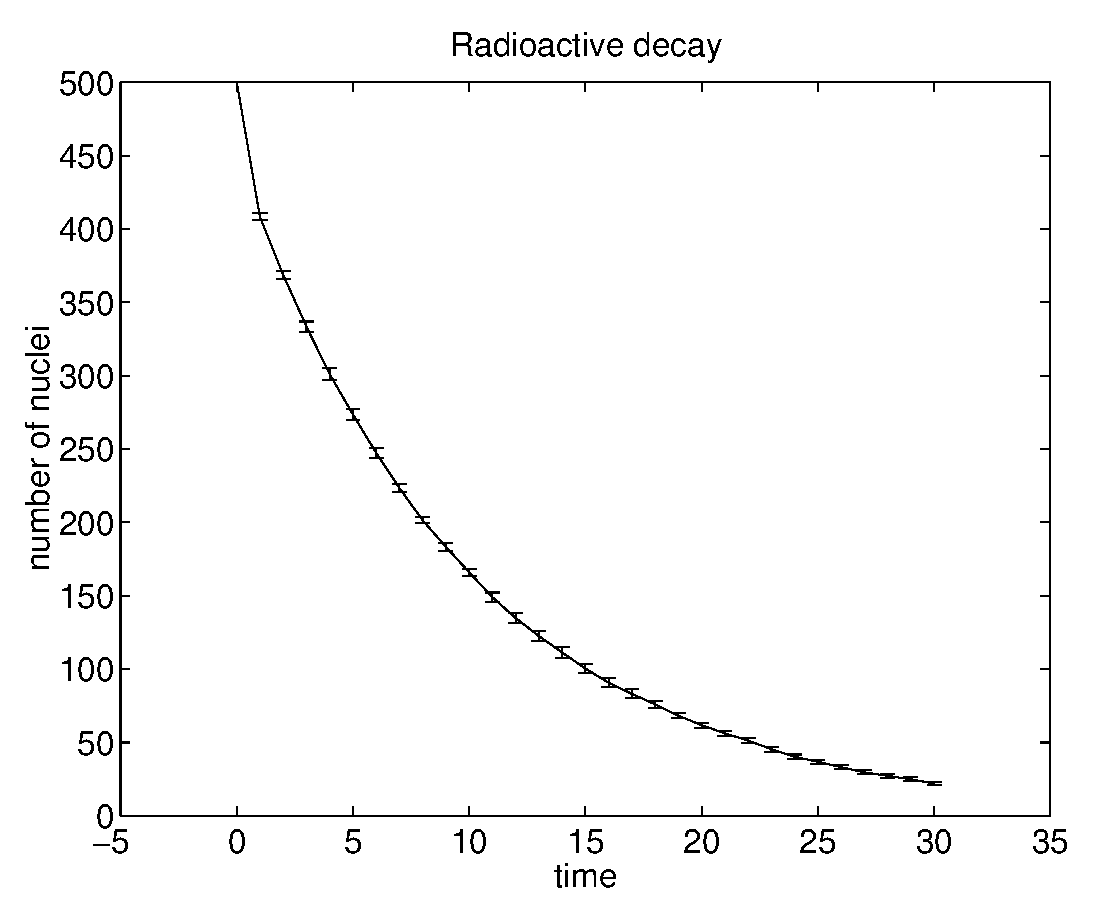
\includegraphics[width=10cm]{./Figures/f_os_decay.eps}
\caption{Stochastic simulation of radioactive decay. The initial
  number of decaying nuclei is {\texttt n0}$= 100$. {\texttt tend}
is 30 and the ensemble average was taken over 10 realizations.
The decay rate is $\gamma=0.1$.}
\end{figure}  

\subsection{The Poisson Process}
A further important one--step process is the Poisson process, which
is defined by
\begin{equation}
r(n) = 0; \;\;\; g(n) = q = \text{const}.
\end{equation}
Inserting the above transition rates into the master equation
(\ref{MASTER_ONE_STEP}) we get the master equation defining
the Poisson process
\begin{equation}
\label{MASTER_POISSON}
\frac{\partial}{\partial t} P(n,t|n',t') =
  q [ P(n-1,t|n',t') - P(n,t|n',t')].
\end{equation}
The Poisson process describes a random walk over the integers
$0,1,2,\ldots$. The steps of the walk are all of length $l$ and are 
only to the right. They are performed at random times with 
probability per unit time equal to $q$.

It is instructive to consider the analytical solution of the 
above master equation (\ref{MASTER_POISSON}). The analytical
solution will be constructive with the help of a very useful 
technique which is based upon the characteristic function
\begin{equation*}
G(s,t) = \langle \exp(ins)\rangle = \sum_n P(n,t|n',t') \exp(ins).
\end{equation*}
The  equation of motion for the characteristic function is easily 
obtained with the help of (\ref{MASTER_POISSON}). We find
\begin{equation*}
\frac{\partial}{\partial t} G(s,t) = 
       q \left[ \exp(is) -1 \right] G(s,t).
\end{equation*}
Assuming that at time $t'$ the one--sided random walk starts at
$n'=0$, the initial condition of the above differential equation
reads
\begin{equation*}
G(s,0) = 1.
\end{equation*}
In this case the solution of the above differential equation of 
motion  for the characteristic function is easily found. It reads
\begin{equation*}
G(s,t) = \exp\left\{ tq \left[ \exp(is)-1 \right]\right\}.
\end{equation*}
To read out the analytical solution for the transition probability
$P(n,t|0,0)$ it is convenient to write the above solution in the
form
\begin{eqnarray*}
G(s,t) &= & \exp(-tq) \exp \left[ tq \exp(is)\right] \\
       &= & \sum_{n=0}^{\infty} \exp(-tq) 
             \frac{[tq\exp(is)]^n}{n!}.
\end{eqnarray*}
For $s=0$ and from the definition of the characteristic function
it follows immediately that
\begin{equation*}
P(n,t|0,0) = \exp(-tq) \frac{(tq)^n}{n!},
\end{equation*}
which evidently is a Poisson distribution. As we know the 
characteristic function allows the determination of all moments of 
the stochastic process through the relation
\begin{equation*}
\langle n^m(t) \rangle = \left. 
       \left( -i \frac{\partial}{\partial s} \right) G(s,t)  
       \right|_{s=0}.
\end{equation*}
Applying the above formula we find
\begin{equation*}
\langle n(t) \rangle = qt
\end{equation*}
and
\begin{equation*}
\langle n^2(t) \rangle = qt + (qt)^2.
\end{equation*}
Accordingly, the variance of the Poisson process is given by
\begin{equation*}
\text{Var}(n) = \langle n^2(t) \rangle - \langle n(t) \rangle^2 = 
   qt.
\end{equation*}
The simulation of the Poisson process is straightforward. We make 
use of the program \texttt{onestep.m} and simply write a new 
function \texttt{poissonmaster.m} according to the 
master equation (\ref{MASTER_POISSON}) whose listing can be
seen below.

\subsubsection{Listing of the function {\texttt{poissonmaster.m}}}
\inputlisting{./Listings/poissonmaster.m}

To begin we generate one realization of the Poisson process. To 
this end we run the program with the following parameters:
\texttt{nstart=0}, \texttt{tend=30}, \texttt{nreal=1}. In the 
function \texttt{poissonmaster} we have chosen the transition rate
to be \texttt{q=1}. One realization of the Poisson process can be
seen in Fig. (\ref{F_OS_POI_R}).
\begin{figure}
\label{F_OS_POI_R}
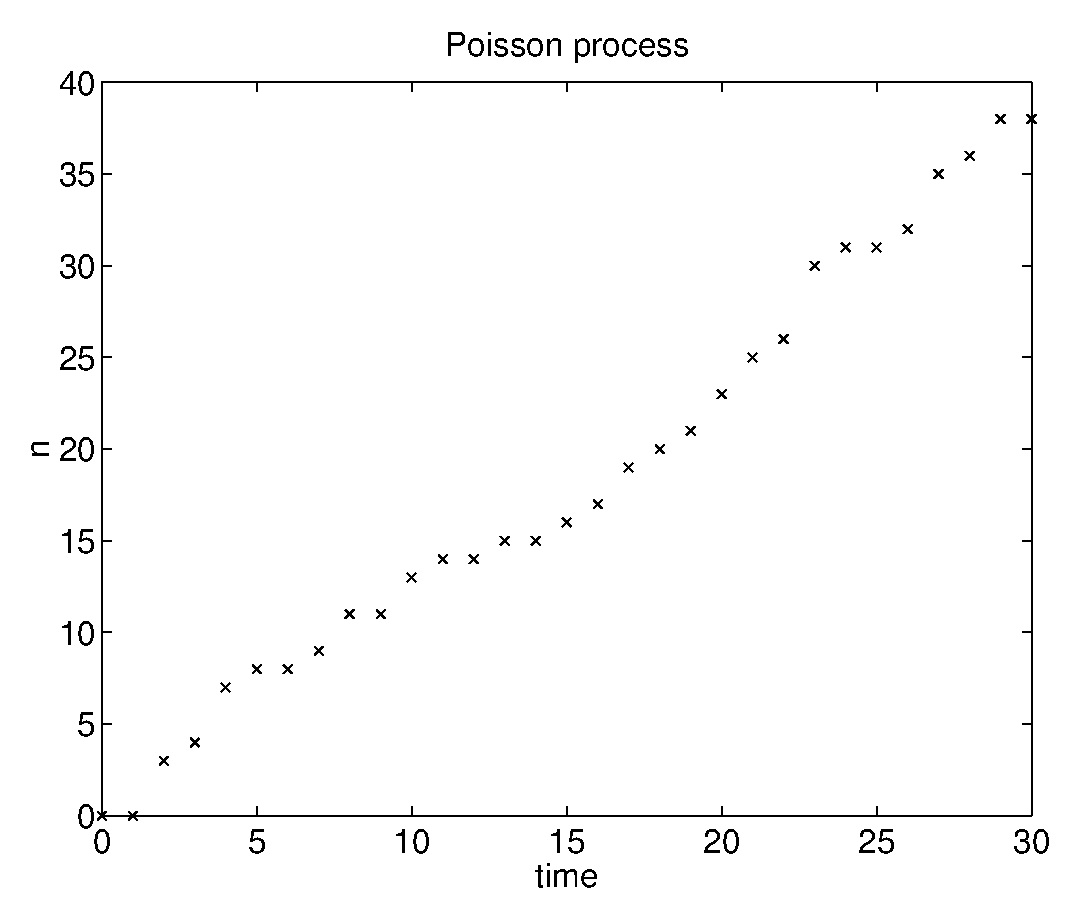
\includegraphics[width=10cm]{./Figures/f_os_poi_r.eps}
\caption{Stochastic simulation of the Poisson process. The 
one--sided random walk starts at \texttt{nstart=0}.  
{\texttt tend} is 30 and \texttt{nreal=1}.
The jump rate is \texttt{q=1}.}
\end{figure}  
In Fig. (\ref{F_OS_POI_1}) we show an ensemble average over 20
realizations of the Poisson process. The other parameters are 
unchanged.
\begin{figure}
\label{F_OS_POI_1}
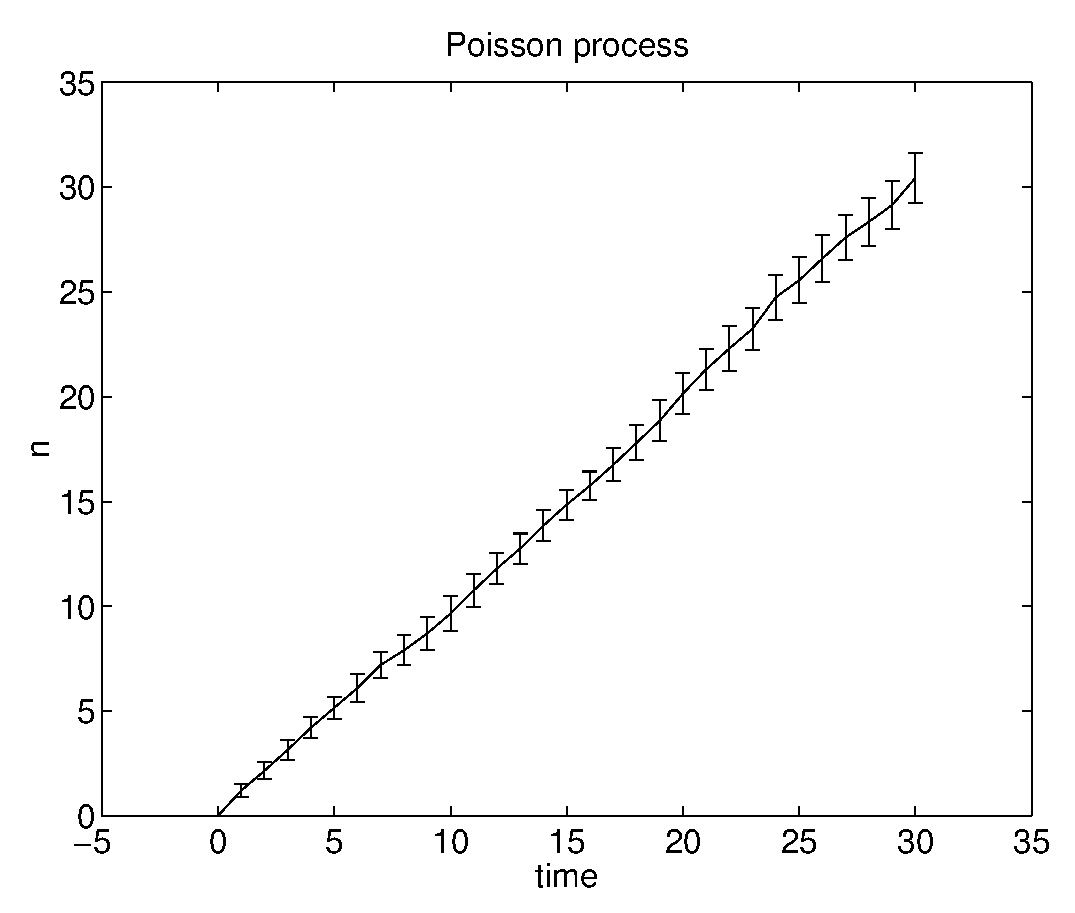
\includegraphics[width=10cm]{./Figures/f_os_poi_1.eps}
\caption{Stochastic simulation of the Poisson process. The 
one--sided random walk starts at \texttt{nstart=0}.  
{\texttt tend} is 30 and \texttt{nreal=20}.
The jump rate is \texttt{q=1}.}
\end{figure}
It is interesting to consider the limit of continuous space for the
Poisson process. Let us denote the distance travelled by 
\begin{equation*}
x=nl.
\end{equation*}
As a function of the new stochastic variable $x$ the 
characteristic function $\tilde{G}$ is
\begin{equation*}
\tilde{G}(s,t) = \langle \exp(isx) \rangle = 
     \exp\{tq[\exp(ils)-1] \}.
\end{equation*}
We perform the limit $l \longrightarrow 0$ keeping 
\begin{equation*}
ql=v=\text{const}
\end{equation*}
and obtain keeping only the terms linear in $l$ in the Taylor
expansion of $\exp(ils)$
\begin{equation*}
\lim_{l\rightarrow 0}\tilde{G}(s,t) = \exp(itvs).
\end{equation*}
So, in the continuum limit the transition probability is
\begin{equation*}
P(x,t|0,0) = \delta(x-vt).
\end{equation*}
Thus, the Poisson process has a deterministic limit. This can also 
be seen by considering, that in the same limit the master equation
for the Poisson process turns into the Liouville equation
\begin{equation*}
\frac{\partial}{\partial t} P(x,t|0,0) = -v 
\frac{\partial}{\partial x} P(x,t|0,0),
\end{equation*}
whose solution is the deterministic process we have just derived.
This behaviour can also be seen in the simulation. To this end
we run the program \texttt{onestep} with the function 
\texttt{poissonmaster} choosing \texttt{q=10}. The result of the 
simulation can be seen in Fig. (\ref{F_OS_POI_2}).
\begin{figure}
\label{F_OS_POI_2}
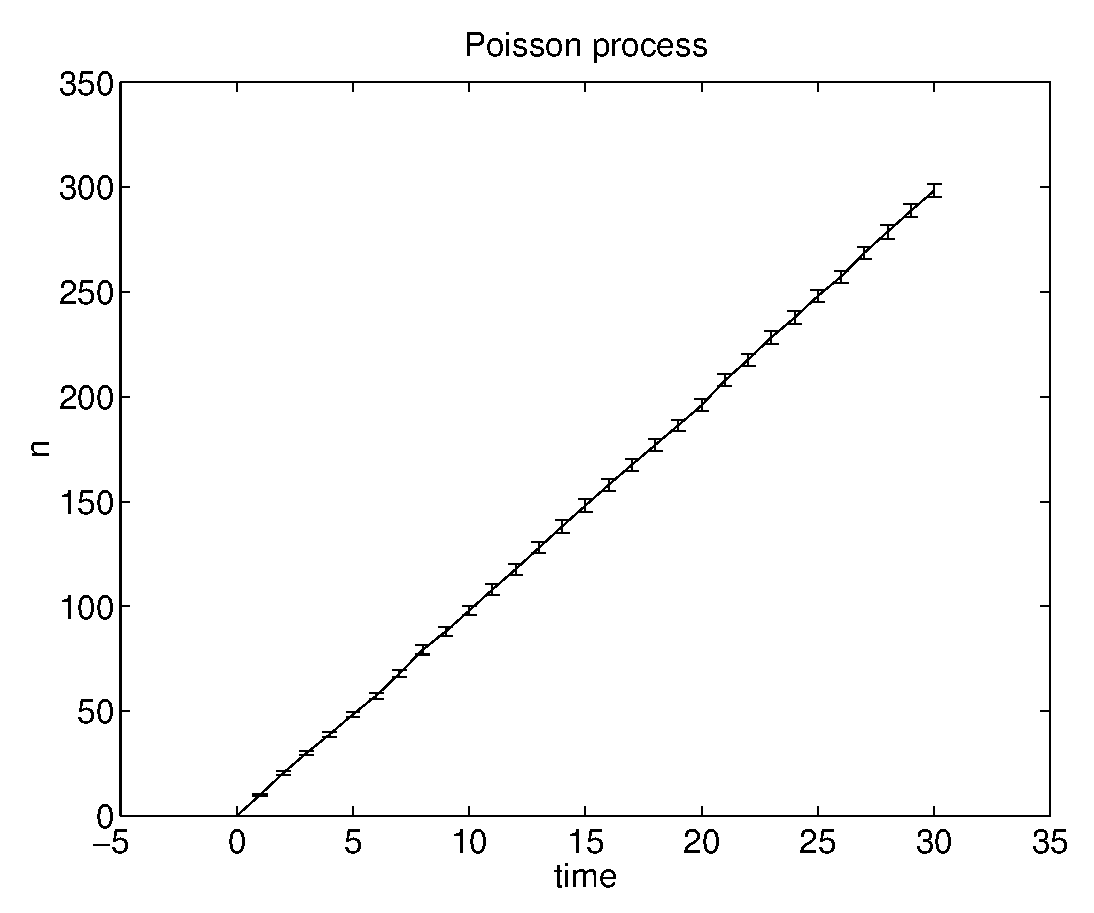
\includegraphics[width=10cm]{./Figures/f_os_poi_2.eps}
\caption{Stochastic simulation of the Poisson process. The 
one--sided random walk starts at \texttt{nstart=0}.  
{\texttt tend} is 30 and \texttt{nreal=20}.
The jump rate is \texttt{q=10}.}
\end{figure}
As we can see for a larger value of \texttt{q} the variance of the
process gets smaller. Thus the dynamics of the process is nearly 
deterministic.

\subsection{The Continuous Time Random Walk}
In this subsection we want to consider the master equation for
the one--dimensional random walk. The steps of the walker are of 
length $l$. The positions of the walker are $nl$ and are labelled
by the integer $n$. We already considered the random walk problem 
in Chapter 2.  There the walker was allowed to take steps 
to the left and to the right at some 
discrete times $N\tau$, where the time step $\tau$ was fixed.
Now, we consider a random walk which is continuous in time. The 
walker is allowed to take steps to the left or to the right with 
the probability per unit time $q$. This process is again described 
by a master equation for a one--step process (\ref{MASTER_ONE_STEP})
by choosing
\begin{equation*}
r(n) =g(n) =q.
\end{equation*}
Thus the master equation for the continuous time random walk
reads
\begin{eqnarray}
\label{MASTERWALK}
\frac{\partial}{\partial t} P(n,t|n',t') &=& 
       q \left\{ P(n+1,t|n',t') + P(n-1,t|n',t')\right. \\
       && \left.  - 2 P(n,t|n',t')  \right\}. \nonumber
\end{eqnarray}
Again the above master equation is easily solved with the help of 
the characteristic function $G(s,t)$. It is easy to check that the
characteristic function satisfies the equation
\begin{equation*}
\frac{\partial}{\partial t} G(s,t) = q [\exp(is) +\exp(-is) -2] G(s,t).
\end{equation*}
Assuming that the walker starts at time $t'=0$ in $n'=0$ we find
$G(s,0)=1$ and the solution of the above equation reads
\begin{equation*}
G(s,t) = \exp\{[ \exp(is) +\exp(-is) -2  ]tq\}.
\end{equation*}
With the help of the above expression for the characteristic 
function the moments are easily evaluated. We find
\begin{eqnarray*}
\langle n(t) \rangle &=& 0, \\
\langle n^2(t) \rangle &=& 2tq.
\end{eqnarray*}
Again we find the typical behaviour of a diffusive process.

The continuous time random walk is also easily simulated with the
help of the program \texttt{onestep}. To this end we have to write
a new function \texttt{walkmaster.m} which implements the 
appropriate transition rates.

\subsubsection{Listing of the function \texttt{walkmaster.m}}
\inputlisting{./Listings/walkmaster.m}

We run the program with the following parameters: 
\texttt{nstart=0}, \texttt{nreal=10}, \texttt{tend=30}, and
\texttt{q=1}. The result of the simulation can be seen in
Fig. (\ref{F_CTRW}).
\begin{figure}
\label{F_CTRW}
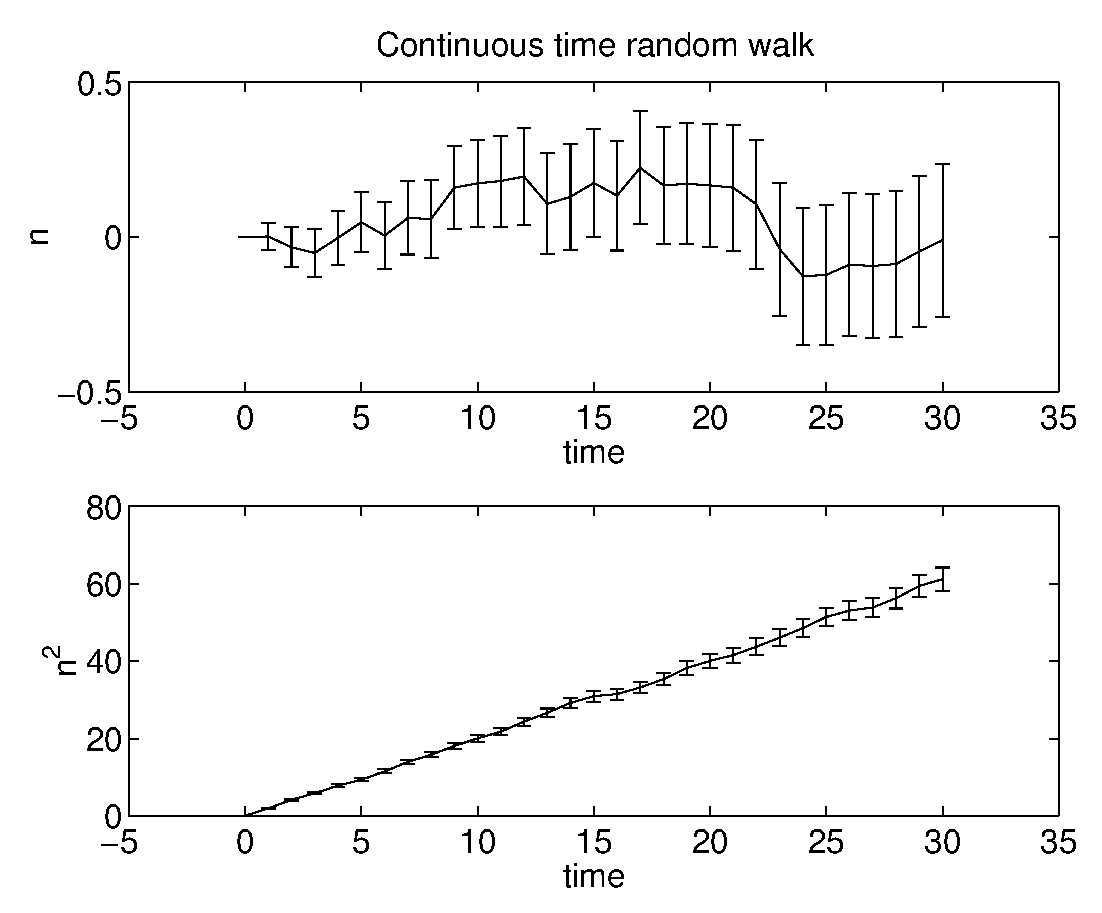
\includegraphics[width=10cm]{./Figures/f_ctrw.eps}
\caption{Stochastic simulation of the continuous time
random walk. The 
random walk starts at \texttt{nstart=0}.  
{\texttt tend} is 30 and \texttt{nreal=20}.
The jump rate is \texttt{q=1}.}
\end{figure}

It is of particular interest to look at the continuous space limit
of the continuous time random walk. Again we write for the 
distance travelled by the walker $x=nl$. The characteristic
function as a function of $x$ reads
\begin{eqnarray*}
\tilde{G}(s,t) &=& G(sl,t) = \langle \exp(ixs) \rangle \\
                &=& \exp\{[\exp(ils) + \exp(-ils)-2]tq \}.
\end{eqnarray*}
The limit of infinitesimally small steps $l \longrightarrow 0 (ql=\text{const.})$ 
leads to
\begin{equation}
\label{CHAR_WALK_X}
\tilde{G}(s,t) = \exp(-s^2tD),
\end{equation}
where
\begin{equation*}
D=\lim_{l\rightarrow 0} (l^2q).
\end{equation*}
The quantity $D$ can be interpreted as the mean square distance 
traveled  per unit time.  The characteristic function (\ref{CHAR_WALK_X})
is the characteristic function of a Gaussian process of the form
\begin{equation*}
P(x,t|0,0) = \frac{1}{(4\pi Dt)^{1/2}} \exp\left( -x^2/4Dt 
\right).
\end{equation*}
This is the transition probability of a so--called {\em Wiener process},
which can be regarded as a continuous time random walk in the 
limit of infinitesimally small step size. We will consider the 
Wiener process in more detail in the next section.

The following remark may serve as an introduction to the next 
section. Of course, we can also expand directly the master equation
(\ref{MASTERWALK}) as a function of $x$ up to second order terms 
in $l$ and get
\begin{equation*}
\frac{\partial}{\partial t} P(x,t|0,0) =
     (l^2q) \frac{\partial^2}{\partial x^2} P(x,t|0,0),
\end{equation*}
which is a special type of Fokker--Planck equation, as we will see 
in the next section.

\section{The Fokker--Planck Equation}
In this section we want to derive the Fokker--Planck equation
(\cite{RISKEN}),
which is a special type of master equation (\cite{VAN_KAMPEN})
in the limit of small jumps.
We begin by expressing the transition probability $w$ as a 
function of the size $r$ of the jump and of the starting point
\begin{equation*}
w(y,y') = w(y';r); \;\;\; r=y-y'.
\end{equation*}
The master equation (\ref{MASTER_JUMP_P}) then reads
\begin{equation}
\label{MASTER_SMALL_JUMP}
\frac{\partial}{\partial t} P(y,t) =
  \int dr w(y-r;r)P(y-r,t) - \int dr w(y;-r)P(y,t).
\end{equation}
In order to consider the limit of small jumps essentially
two assumptions will be needed. The first is that
the function
$w(y;r)$ will be a sharply peaked function of $r$ and will
vary slowly with $y$. To be more precise we assume that a $\delta >0$
exists such that
\begin{eqnarray*}
w(y';r)  & \approx & 0 \;\;\; \text{for} \;\;\; |r|> \delta \\
w(y'+\Delta y;r) & \approx & w(y';r) \;\;\; \text{for} \;\;\; |\Delta y| < 
\delta.
\end{eqnarray*}
The second assumption is that the solution $P(y,t)$ of the master equation 
in this limit will be a slowly varying function of $y$.

If these assumptions hold it is safe to expand the shift from $y$
to $y-r$ in the first integral in 
Eq. (\ref{MASTER_SMALL_JUMP}) in a Taylor series
\begin{equation}
\label{MASTER_EXPAND}
\frac{\partial}{\partial t} P(y,t) = \sum_{\nu=0}^{\infty}
   \frac{(-1)^{\nu}}{\nu!} \left( \frac{\partial}{\partial y} 
   \right)^{\nu}
    \left\{  a_{\nu}(y) P(y,t) \right\}
    - P(y,t) \int_{-\infty}^{\infty} dr w(y;-r),
\end{equation}
where we have defined
\begin{equation*}
a_{\nu}(y) = \int_{-\infty}^{\infty} dr r^{\nu} w(y;r).
\end{equation*}
Since the zeroth term in the sum and the second term of 
Eq. (\ref{MASTER_EXPAND}) cancel the small jumps expansion 
of the master equation reads
\begin{equation}
\frac{\partial}{\partial t} P(y,t) = \sum_{\nu=1}^{\infty}
   \frac{(-1)^{\nu}}{\nu!} \left( \frac{\partial}{\partial y} 
   \right)^{\nu}
    \left\{  a_{\nu}(y) P(y,t) \right\}.
\end{equation}
The above expansion is called the Kramers--Moyal expansion. 
Formally, we can write
\begin{equation}
\frac{\partial}{\partial t} P(y,t) = {\cal{A}}_{KM}^{\dagger}(y)
         P(y,t),
\end{equation}
where we introduced the adjoint generator
\begin{equation*}
{\cal{A}}_{KM}^{\dagger}(y) = \sum_{\nu=1}^{\infty}
   \frac{(-1)^{\nu}}{\nu!} \left( \frac{\partial}{\partial y} 
   \right)^{\nu}
     a_{\nu}(y).
\end{equation*}
It is easy to show by partial integration that the corresponding
generator  reads
\begin{equation*}
{\cal{A}}_{KM}(y) = \sum_{\nu=1}^{\infty}
   \frac{1}{\nu!}  a_{\nu}(y)
    \left( \frac{\partial}{\partial y} 
   \right)^{\nu}.
\end{equation*}
It is clear that dealing with the {\em Kramers--Moyal} expansion will 
not be easier than dealing with the original master equation.

A particularly interesting and useful approximation to a jump process is 
obtained by keeping only terms up to the second order in $\nu$
\begin{equation}
\label{FOKKER_PLANCK}
\frac{\partial}{\partial t} P(y,t) =
-\frac{\partial}{\partial y} \left\{ a_1(y) P(y,t) \right\}
   + \frac{1}{2} \frac{\partial^2}{\partial y^2} 
      \left\{ a_2(y) P(y,t) \right\}.
\end{equation}
The above equation is called the {\em Fokker--Planck equation}.
The first term on the right--hand side is usually called the drift
term since it is essentially Liouvillian. The second term
on the right--hand side is the diffusion term. In a later section
we will learn how to deal with this equation.

\subsection{The Wiener Process}
\label{sec:WienerProcess}
Let us consider the important special case 
of vanishing drift, i.e. $a_1=0$, and diffusion coefficient
equal to one, i.e. $a_2=1$. The generator takes the form 
\begin{equation}
\label{WIENER_GENERATOR}
{\cal{A}}_W = {\cal{A}}_W^{\dagger} = \frac{1}{2} 
     \frac{\partial^2}{\partial y^2},
\end{equation}
and it defines a Wiener process. We already met the corresponding
Fokker--Planck equation, 
when we considered the continuous space limit of the the 
continuous time random walk.
Now we want to write down this Fokker--Planck equation in the form
\begin{equation*}
\frac{\partial}{\partial t}T(w,t|w_0,t_0) =
  \frac{1}{2} \frac{\partial^2}{\partial x^2} T(w,t|w_0,t_0).
\end{equation*}
The above equation can easily be solved with the help of the 
characteristic function
\begin{equation*}
G(s,t) = \int dw T(w,t|w_0,t_0) \exp(isw),
\end{equation*}
where we have assumed that the initial condition on the transition 
probability is
\begin{equation*}
T(w,t_0|w_0,t_0) = \delta(w-w_0).
\end{equation*}
The characteristic function satisfies the equation
\begin{equation*}
\frac{\partial}{\partial t}G(s,t) = - \frac{1}{2} s^2 G(s,t),
\end{equation*}
whose solution is, given the initial condition $G(s,t_0)=\exp(isw_0)$, 
\begin{equation*}
G(s,t) = \exp\left[isw_0 -s^2(t-t_0)/2\right].
\end{equation*}
Performing the inverse Fourier transformation of the above 
expression we find the transition probability
\begin{equation}
\label{TRANS_WIENER}
T(w,t|w_0,t_0)= \frac{1}{[2 \pi (t-t_0)]^{1/2}}
     \exp\left[ -(w-w_0)^2/2(t-t_0)\right].
\end{equation}
Thus, the transition probability density is a Gaussian with
\begin{eqnarray*}
\langle W(t) \rangle &=& w_0 \\
\langle [W(t)-w_0]^2\rangle &=& t-t_0.
\end{eqnarray*}
An initially sharp peaked distribution spreads in time.
It is important to make some remarks on the Wiener process $W(t)$.

The mean square of the Wiener process diverges linearly with time.
As we already know this behaviour is typical for diffusion 
processes and the trajectories of the Wiener process are very 
variable. We will look at the trajectories of the Wiener process 
soon. 

Although the paths of the Wiener process are continuous they are 
not differentiable since the derivative at any point is 
almost certainly infinite (\cite{gardiner}).

The Wiener process plays a central role in the description of 
diffusion processes by means of stochastic differential equations.
The reason is that the increments of the Wiener process
\begin{equation*}
\Delta W_i \equiv W(t_i) - W(t_{i-1}) \equiv W_i -W_{i-1} 
\end{equation*}
are statistically independent. This can be seen in the following 
way. Let us consider the joint probability density
\begin{eqnarray*}
P(w_n,t_n; w_{n-1},t_{n-1}; \ldots ; w_0,t_0) &=&
\prod_{i=0}^{n-1} T(w_{i+1},t_{i+1}|w_i,t_i) P(w_0,t_0).
\end{eqnarray*}
Exploiting the explicit form of the transition probabilities
(\ref{TRANS_WIENER}) the above joint probability density can be 
cast in the following form
\begin{eqnarray*}
\lefteqn{P(w_n,t_n; w_{n-1},t_{n-1}; \ldots ; w_0,t_0) =} \\
& & \prod_{i=0}^{n-1} 
\left\{ \frac{1}{[2 \pi (t_{i+1}-t_i)]^{1/2}}
\exp[-(w_{i+1}-w_i)^2/2(t_{i+1}-t_i)]
\right\}
P(w_0,t_0).
\end{eqnarray*}
Expressed in terms of the increments $\Delta W_i$ the above 
equation reads
\begin{eqnarray*}
\lefteqn{
P(\Delta w_n,\Delta t_n; \Delta w_{n-1},\Delta t_{n-1}; \ldots ; w_0,t_0) =} \\
& &\prod_{i=1}^{n} 
\left\{ \frac{1}{[2 \pi \Delta t_i)]^{1/2}}
\exp[-\Delta w_i^2/2 \Delta t_i]
\right\}
P(w_0,t_0),
\end{eqnarray*}
where we have introduced the variables
\begin{equation*}
\Delta t_i = t_{i} - t_{i-1}.
\end{equation*}
Thus, the increments $\Delta W_i$ are evidently statistically
independent and are distributed according to
\begin{equation*}
P(\Delta w,\Delta t) = \frac{1}{[2 \pi \Delta t)]^{1/2}}
\exp[-\Delta w^2/2 \Delta t].
\end{equation*}

At this point it is convenient to introduce a short hand notation 
for Gaussian distributed random numbers. The Gaussian random 
variable $X$ with mean $m$ and variance $\sigma^2$ will be denoted
by
\begin{equation*}
X \equiv {\bf N}(m,\sigma^2).
\end{equation*}
In particular we will name the random variable $\xi$
\begin{equation*}
\xi \equiv {\bf N}(0,1)
\end{equation*}
the unit normal random variable. In this notation we can write
for the Wiener $W(t)$ process
\begin{equation*}
W(t) = {\bf N} ( W_0, (t-t_0) )
\end{equation*}
and for the increment $\Delta W$
\begin{equation*}
\Delta W(t) = {\bf N} (0, 
     \Delta t ).
\end{equation*}

For later convenience we give two rules concerning the 
transformation of Gaussian random variables. First, let $a$ and $b$
be two numbers, then we have
\begin{equation*}
a +b {\bf N}(m,\sigma^2) = {\bf N} ( a+bm, b^2\sigma^2).
\end{equation*}
In particular we have for a unit normal random variable
\begin{equation*}
a+b\xi = {\bf N}(a,b^2).
\end{equation*}
Second, if ${\bf N}(m_1,\sigma_1^2)$ and ${\bf N}(m_2,\sigma_2^2)$ 
are statistically independent, then
\begin{equation*}
{\bf N}(m_1,\sigma_1^2) + {\bf N}(m_2,\sigma_2^2) =
   {\bf N}(m_1+m_2,\sigma_1^2+\sigma_2^2).
\end{equation*}
The above rule expresses the fact that, as we know, that Gaussian 
random variables remain Gaussian distributed under addition.
The rules just given can be demonstrated with the help of the 
random variable transformation theorem.

With the help of the first above rule it is clear that the 
increment $\Delta W$ can be expressed as
\begin{equation*}
\Delta W = \sqrt{\Delta t} \xi,
\end{equation*}
where $\xi$ is the unit normal random variable.

Let us now generate numerically some realizations of the Wiener 
process. To this end we need a way of calculating for a given 
value of the Wiener process $W(t)$ at time $t$ the value of the
process at time $t+\Delta t$. We will present an algorithm which
is exact for any positive value of $\Delta t$ (\cite{GILLESPIE}).

The algorithm exploits the fact that we know analytically the
conditional transition probability density. $T(w,t|w',t')$ is a 
Gaussian  with  mean $w'$ and variance $\sigma^2=2(t-t')$.
Accordingly, given $W(t)$ the increment $\Delta W(t)$
\begin{equation}
\label{ADVANCE_WIENER}
W(t+\Delta t) = W(t) + \Delta W(t)
\end{equation}
is distributed according to a Gaussian with zero mean and variance
$\sigma^2=2\Delta t$. The above formula is the update formula
for the algorithm for the generation of realizations of the Wiener
process. The algorithm essentially consists of the following 
steps:

(i) Let $W(t)$ be given.

(ii) Draw a Gaussian distributed random number $\Delta W$
with zero mean and variance $\sigma^2=2\Delta t$).

(iii) Advance the stochastic process according to the formula
(\ref{ADVANCE_WIENER}).

(iv) Goto (i) until the desired final time is reached.

A flow diagram of the program \texttt{wiener.m} can be seen in 
Fig. (\ref{F_WIENER_ALGORITHM}). 
\begin{figure}
\label{F_WIENER_ALGORITHM}
\includegraphics[width=6cm]{./Figures/f_wiener_algorithm.eps}
\caption{Flow diagram of the program \texttt{wiener.m}}
\end{figure}
\subsubsection{Listing of the function \texttt{wiener.m}}
\inputlisting{./Listings/wiener.m}

Let us run the program two times with the following parameters
\texttt{xstart=0}, \texttt{tend=50}, \texttt{deltat=0.01}, 
\texttt{nreal=1} in order to generate two realizations of the 
Wiener process. The two independent realizations can be seen 
on Figs. (\ref{F_WIENER_R1}) and (\ref{F_WIENER_R2}). The great 
variability of the realizations is evident. 
\begin{figure}
\label{F_WIENER_R1}
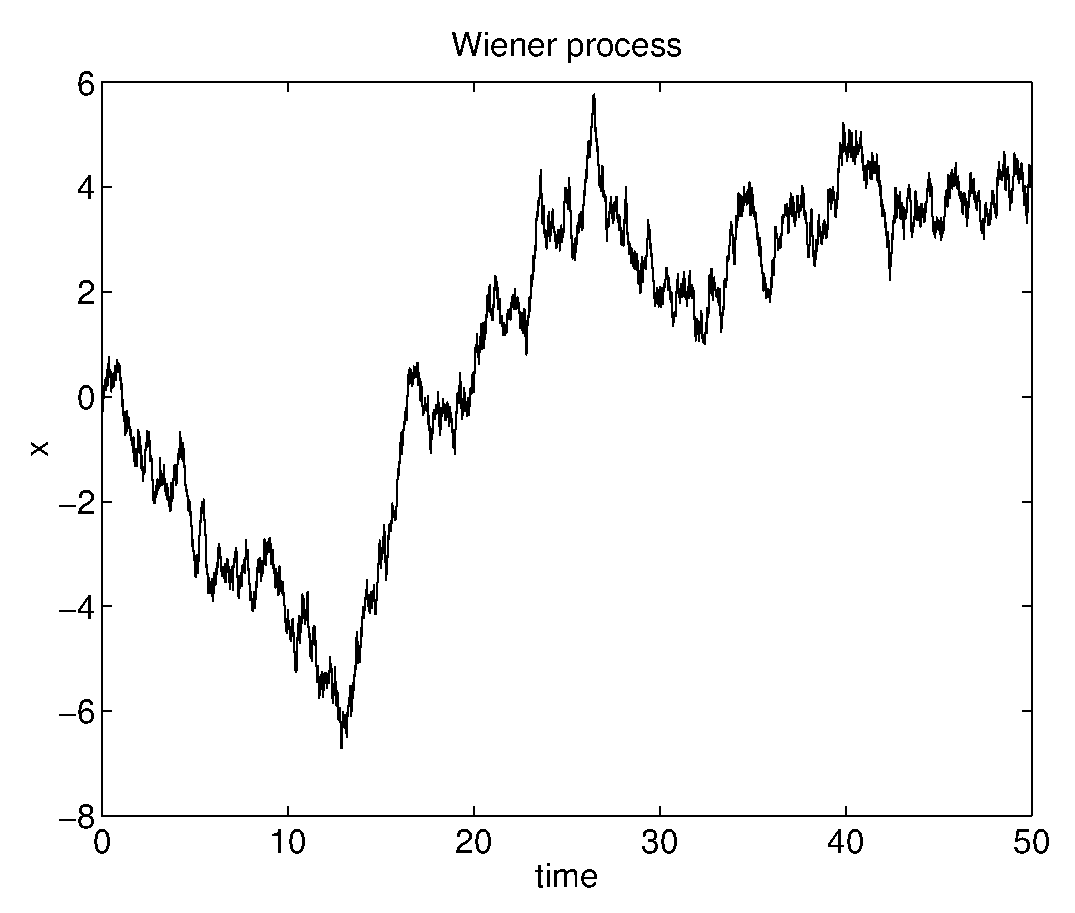
\includegraphics[width=10cm]{./Figures/f_wiener_r1.eps}
\caption{One realization of the Wiener process.
The parameters used in the simulation are \texttt{xstart=0},
\texttt{tend=50}, \texttt{deltat=0.01}, and \texttt{nreal=1}.}
\end{figure}
\begin{figure}
\label{F_WIENER_R2}
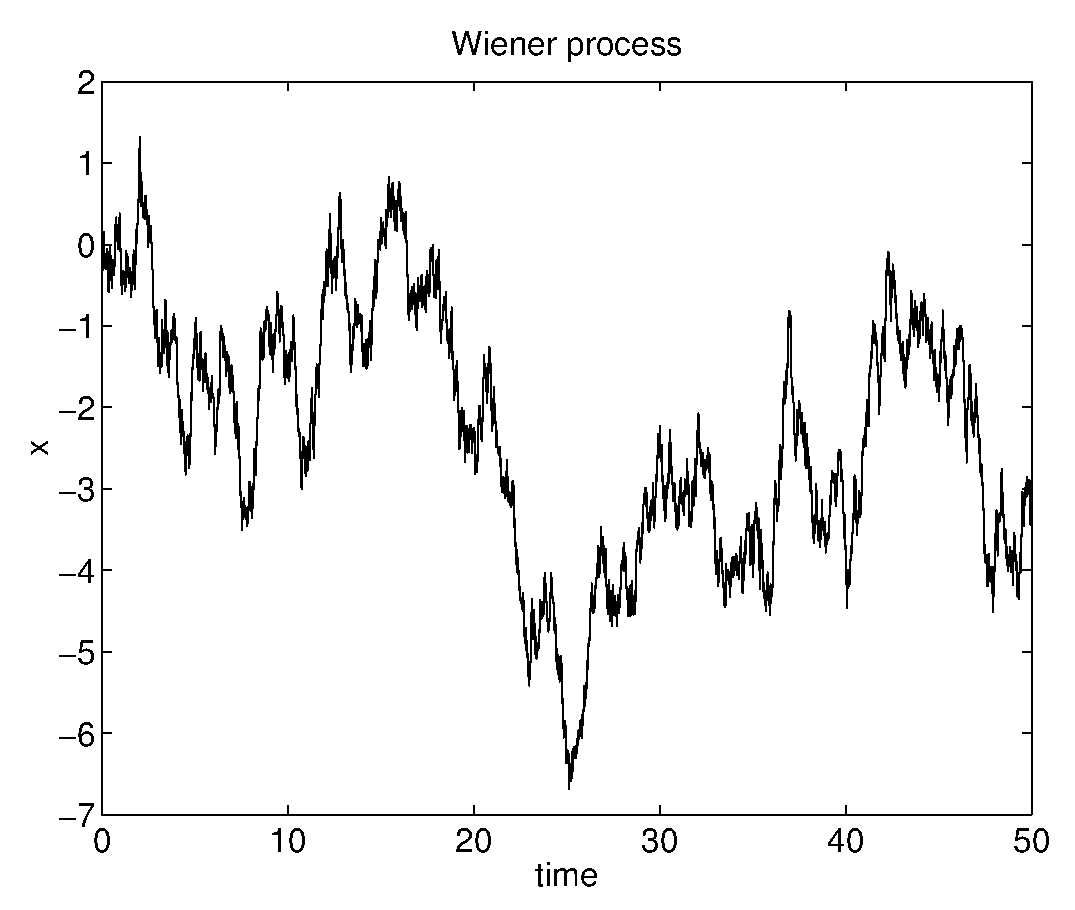
\includegraphics[width=10cm]{./Figures/f_wiener_r2.eps}
\caption{One realization of the Wiener process.
The parameters used in the simulation are \texttt{xstart=0},
\texttt{tend=50}, \texttt{deltat=0.01}, and \texttt{nreal=1}.}
\end{figure}
In Fig. (\ref{F_WIENER}) we show an ensemble average of the
Wiener process over 1000 realizations.
\begin{figure}
\label{F_WIENER}
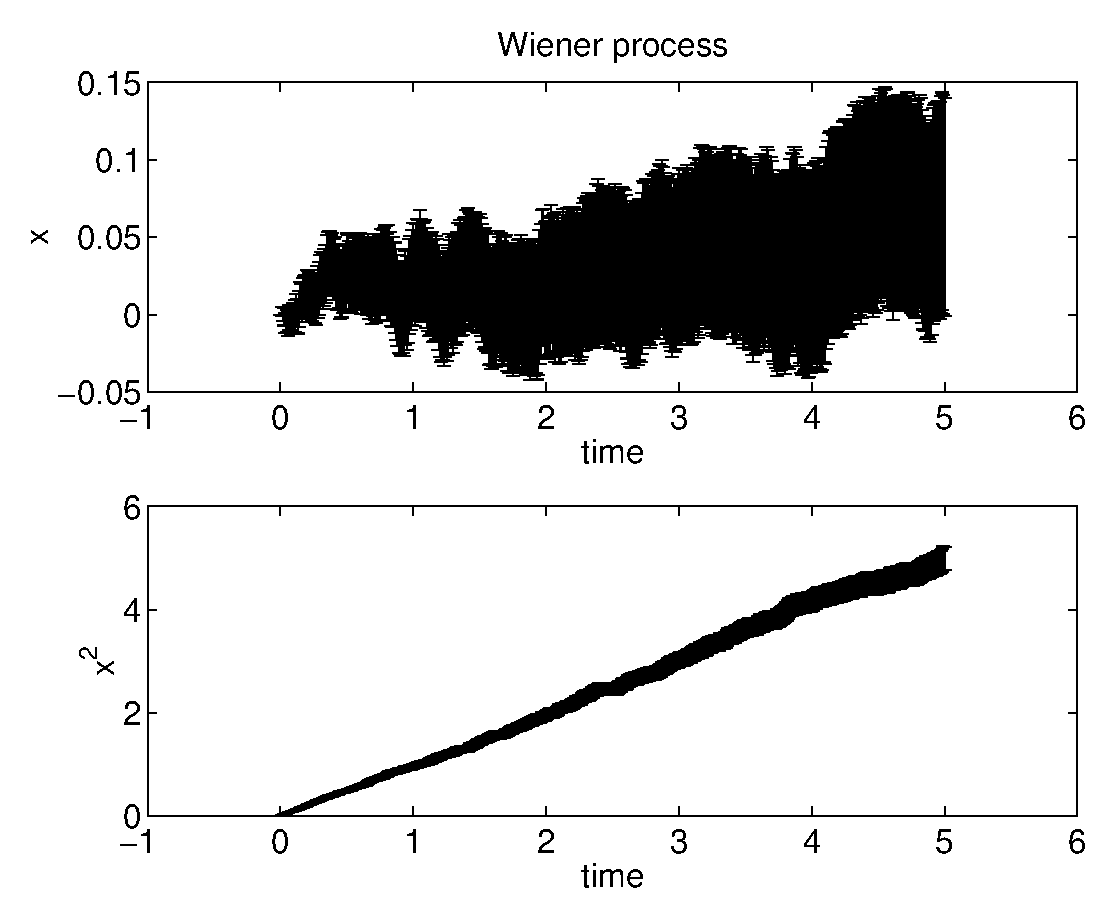
\includegraphics[width=10cm]{./Figures/f_wiener.eps}
\caption{One realization of the Wiener process.
The parameters used in the simulation are \texttt{xstart=0},
\texttt{tend=5}, \texttt{deltat=0.01}, and \texttt{nreal=1000}.}
\end{figure}

\subsection{The Ornstein--Uhlenbeck Process}
Up to now we have considered only Fokker--Planck equations 
without drift. 
As a simple example of a Fokker--Planck equation with an 
additional linear drift we consider
\begin{equation}
\label{ORNSTEIN}
\frac{\partial}{\partial t} T(x,t|x',t') = 
\frac{\partial}{\partial x} [qx T(x,t|x',t')] 
+ \frac{1}{2} D \frac{\partial^2}{\partial x^2} T(x,t|x',t').
\end{equation}
The above Fokker--Planck equation defines the Ornstein--Uhlenbeck
process. 

Again, we can look at the equation of motion for the characteristic
function of the Ornstein--Uhlenbeck process
\begin{equation*}
G(s,t) = \int_{-\infty}^{\infty} dx \exp(isx) T(x,t|x',t').
\end{equation*}
The equation reads
\begin{equation*}
\frac{\partial}{\partial t}G(s,t) = -qs \frac{\partial}{\partial s} 
G(s,t) - \frac{1}{2} Ds^2 G(s,t).
\end{equation*}
The above partial differential equation may be solved by the 
method of characteristics (\cite{gardiner}). Its solution
for $T(x,t_0|x_0,t_0)=\delta(x-x_0)$ requires the
initial condition 
\begin{equation*}
G(s,0) = \exp(ix_0s)
\end{equation*}
and reads
\begin{equation*}
G(s,t) = \exp\left[ -\frac{Ds^2}{4q}[1-\exp(-2q(t-t_0))] + 
 isx'\exp(-q(t-t_0)) 
\right].
\end{equation*}
Hence, the transition probability $T(x,t|x',0)$ is a Gaussian
with mean
\begin{equation}
\label{MEAN_ORNSTEIN}
\langle X(t) \rangle = x_0\exp(-q(t-t_0))
\end{equation}
and variance
\begin{equation}
\label{VAR_ORNSTEIN}
\text{Var} \{ X(t) \} = \frac{D}{2q} [1- \exp(-2q(t-t_0))].
\end{equation}
Since the Ornstein--Uhlenbeck process is a Gaussian process we can write
\begin{equation*}
X(t) = {\bf N}\left(X_0\exp(-2q(t-t_0)), 
     \frac{D}{2q} (1-\exp(-2q(t-t_0)) ) \right).
\end{equation*}
In contrast to the Wiener process the Ornstein--Uhlenbeck process
has a stationary distribution in the limit $t\longrightarrow \infty$
which is a Gaussian with zero mean and variance $D/2q$.



We now turn to the numerical simulation of realizations of the 
Ornstein--Uhlenbeck process. The problem is to find a way of
determining  from the value of the process $X$ at time $t$
its value at a later time $t+\Delta t$. As for the generation of 
trajectories of the Wiener process it is possible to construct
an update formula for the Ornstein--Uhlenbeck process, which is 
exact for any positive value of the time increment $\Delta t$
(\cite{GILLESPIE96}). In order to derive an update formula we
replace in Eqs. (\ref{MEAN_ORNSTEIN}) and (\ref{VAR_ORNSTEIN})
for the mean and variance of the Ornstein--Uhlenbeck process
$t$ by $t+\Delta t$ and $t_0$ by $t$ and accordingly $x_0$ by
$X(t)$. Since we know that the Ornstein--Uhlenbeck process
is Gaussian distributed it is now clear that the update
formula reads
\begin{equation}
X(t+\Delta t) = X(t) \exp(-qt) 
+ \left[ \frac{D}{2q} [1-exp(-2q\Delta t)] \right]^{1/2} \xi,
\end{equation}
where $\xi$ is a Gaussian distributed random number with zero 
mean and unit variance. Since we know how to generate Gaussian 
distributed random numbers the algorithm for the generation of 
realizations of the Ornstein--Uhlenbeck process with diffusion constant
$D$ and inverse relaxation time $q$ reads

(i) Specify the values of $D$, $q$, $x_0$, $\Delta t$.

(ii) Compute the constant coefficients 
\begin{equation*}
\mu \equiv \exp(-q \Delta t)
\end{equation*}
and
\begin{equation*}
\sigma \equiv \left[ \frac{D}{2q} [1-exp(-2q\Delta t)] 
\right]^{1/2}.
\end{equation*}

(iii) Initialize setting $X=x_0$ and $t=0$.

(iv) Replace $t$ by $t+\Delta t$. Terminate the simulation if $t$
exceeed $t_{\text{end}}$.

(v) Generate a Gaussian distributed random number $\xi$ and 
update the process replacing $X$ by $\mu X + \sigma \xi$.

(vi) Goto (iv).

In figure \ref{fig:FlowOrnstein} we show the flow diagram of the program 
\texttt{ornstein.m} which will be used to generate the 
realizations. The listing of the program can be seen below.
\begin{figure}[htbp]
  \begin{center}
    \label{fig:FlowOrnstein}
%%% ???   \includegraphics[height=\textheight]{Figures/FlowOrnstein.eps}
    \caption{The flow diagram of the simulation of the Ornstein-Uhlenbeck process.} 
  \end{center}
\end{figure}

\subsubsection{Listing of the program \texttt{ornstein.m}}
\inputlisting{./Listings/ornstein.m}

One realization of the Ornstein--Uhlenbeck process generated with 
help of the algorithm we have just constructed can be seen in Fig.
(\ref{F_ORNSTEIN_R})

\begin{figure}
\label{F_ORNSTEIN_R}
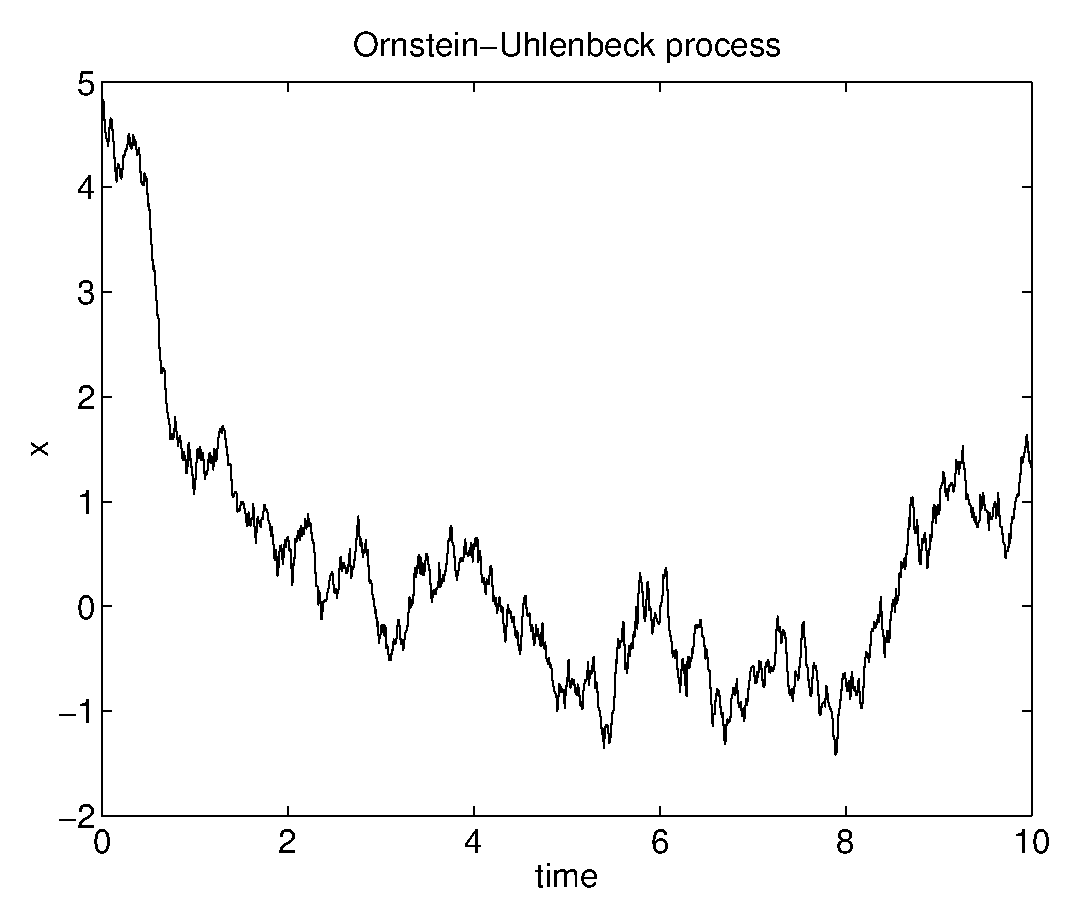
\includegraphics[width=10cm]{./Figures/f_ornstein_r.eps}
\caption{One realization of the Ornstein--Uhlenbeck process. The
 parameters used in the simulation are \texttt{xstart=5},
\texttt{tend=10}, \texttt{deltat=0.01}, \texttt{nreal=1},
\texttt{q=1}, and \texttt{D=1}.}
\end{figure}

The average over 10 realizations of the Ornstein--Uhlenbeck 
process can be seen in Fig. (\ref{F_ORNSTEIN}).
\begin{figure}
\label{F_ORNSTEIN}
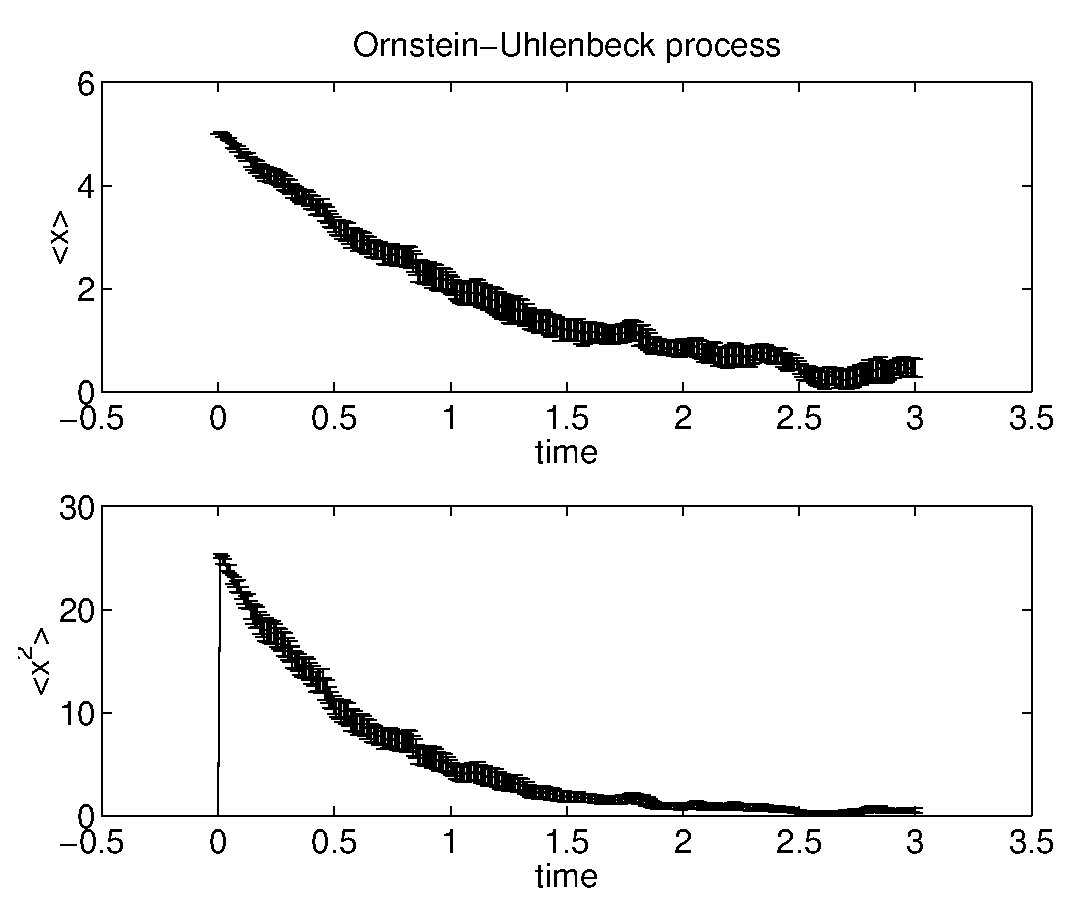
\includegraphics[width=10cm]{./Figures/f_ornstein.eps}
\caption{The average over 10 realizations of the Ornstein--Uhlenbeck 
process. The
 parameters used in the simulation are \texttt{xstart=5},
\texttt{tend=50}, \texttt{deltat=0.01}, \texttt{nreal=10},
\texttt{q=1}, and \texttt{D=1}.}
\end{figure}

%%%%%%%%%%%%%%%%%%%%%%%%%%%%%%%%%%%%%%%%%%%%%%%%%%%%%%%%%%%%%%%%%%%

\section{L\'evy or Stable Distributions}
In this section we address again the problem of the random walk. As we already
know the canonical application of the random walk is the theory of Brownian
motion. The chaotic motion of the Brownian particles over the length scale
$\Delta$  and time scale $\tau$  is modelled by a random walk on a lattice of
spacing $\Delta$, while the steps take place at equal time intervals 
$\tau$. It is the aim of this chapter to go "beyond Brownian motion"
\cite{Klafter:PhysicsToday} and to look at fractal generalizations of
Brownian motion which have proven to be a rich field in probability theory,
statistical physics, chaotic dynamics, and, last not least, in economics.  

We know already that from a mathematical point of view  
the problem of the random walk is the problem of the addition of independent
(usually identically distributed) random variables. For example, if the
individual steps in a one--dimensional walk have displacement $\mu$ and
variance $\sigma^2$, then a simple application of the Central Limit Theorem
tells us that the asymptotic probability density function $P_n$  
for the position $X_n$ after $n$ steps  is given by the Gaussian density with
mean $n\mu$ and variance $n\sigma^2$:
\begin{displaymath}
  P_n(x) \approx \frac{1}{\sqrt{2 \pi n \sigma^2}} \exp 
         \left\{ - \frac{(x- n\mu)^2}{2 n \sigma^2} \right\}.
\end{displaymath}
This is the basic idea of the random walk.  To put it differently, the Central
Limit Theorem states, that if $X_1$, \ldots, $X_N$ are Gaussian distributed
random variables with zero mean and variance $\sigma^2$, the new stochastic
variable 
\begin{displaymath}
  X = \frac{1}{\sqrt{N}} \sum_{i=1}^N X_i
\end{displaymath}
has the same probability density function as the $X_i$.
Now let us consider a slight generalization of the random walk. We consider
an $N$--step random walk in one dimension, with each step of length $x$
governed by the same probability density $p(x)$, with zero mean. Note, that we
expressively do not make any assumption about the variance! The French
mathematician Paul L\'evy \footnote{Paul L\'evy (186--1971)} posed the
following question: When does the probability $P_N(X)$ for the sum of the
steps
\begin{displaymath}
  X = X_1 + X_2 + \cdots + X_N
\end{displaymath}
in general have the same distribution $p(x)$ (up to a scale factor) 
as the individual
steps? As remarked in \cite{Klafter:PhysicsToday} this is the fundamental
question of fractals: When does the whole look like its parts?

??? Abschnitt unverstaendlich !!!
Of course, we already know two answers to the above question.  
As we just recalled in the introductory remarks 
$p(x)$ may be  a
Gaussian density. And we know already that $p(x)$ may be a Cauchy density
\begin{displaymath}
\frac{1}{\pi} \frac{c}{c^2 + (x-\gamma)^2}
\end{displaymath}
(recall that we have have demonstrated in Chap. ??, 
that the sum of two Cauchy variables
is again a Cauchy variable). 
As L\'evy has proved there exist other solutions.
The remarkable aspect of these other solutions is that, as it is the case for
the Cauchy density, all involve random
variables with infinite variance!

The solutions that L\'evy found are called stable (or L\'evy) distributions.
They play a constantly increasing role as a generalization of the normal
distribution. In order to describe stable distributions and look at some of
their properties we follow \cite{Feller2} and introduce the convenient
notation 
\begin{displaymath}
  U {d \atop =} V
\end{displaymath}
to indicate that the random variables $U$ and $V$ have the same distribution.
Throughout this section $X$, $X_1$, $X_2$, \ldots , $X_N$ denote mutually
independent random variables with a common distribution, say $R$ and 
$S_N = X_1 + \cdots + X_N$.

A distribution $R$ is called stable if for each $N$ there exist constants
$c_N >0$ and $\gamma_N$ such that
\begin{equation}
\label{eq:StableDef}
  S_N {d \atop =} c_N  X + \gamma_N.
\end{equation}
The distribution $R$ is called stable in the strict sense if 
(\ref{eq:StableDef}) holds with $\gamma_N =0$. 
The above definition can also be formulated equivalently in the following
form: $R$ is stable if to arbitrary constants $c_1$,  $c_2$  there exist
constants $c$ and $\gamma$ such that
\begin{displaymath}
  c_1 X_1 + c_2 X_2 {d \atop =} c X + \gamma.
\end{displaymath}

Let us now look at some basic properties of stable distributions. 
For a proof of the statements that follow we refer the reader to 
\cite{Feller2}.
The most
important one is that the norming constants $c_N$ in Eq. (\ref{eq:StableDef})
are of the form
\begin{displaymath}
  c_N = N^{1/\alpha},
\end{displaymath}
with  $0< \alpha \le 2$. The constant $\alpha$ is called the
characteristic exponent of the stable distribution  $R$. Sometimes it is also
named the stability index.

An important property is that in practice the  centering constants
$\gamma_N$ may be disregarded. The reason for this fact is that we are free to
center the distribution $R$ in an arbitrary manner, that is, we can replace
$R(x)$ by $R(x+b)$. In fact, if $R$ is stable with an exponent $\alpha \ne 1$
the centering constant $b$ may be chosen so that $R(x+b)$ is strictly stable.
To see why this is so we consider the random variable $S_{MN}$, which is a sum
of $M$ independent variables each distributed according to $c_N X + \gamma_N$,
i.e.,
\begin{equation}
  \label{eq:defSmn}
  S_{MN} = \sum_{i_1}^{N} c_N X_i + \gamma_N.
\end{equation}
So we have
\begin{equation}
  \label{eq:Smn}
  S_{MN} {d \atop =}  c_N S_M + M \gamma_N {d \atop =} c_N c_M X +
                      c_N \gamma_M + M \gamma_N.
\end{equation}
Since $M$ and $N$ play the same role it follows from (\ref{eq:defSmn}) and 
(\ref{eq:Smn}) that
\begin{displaymath}
  (c_N -N) \gamma_M = (c_M -M) \gamma_N.
\end{displaymath}
For $\alpha =1$ the above equation does not have a solution, but when $\alpha
\ne 1$ it implies that
\begin{displaymath}
  \gamma_N = b(c_n -N) 
\end{displaymath}
for all $N$. It follows now from Eq. (\ref{eq:StableDef}) that the sum
$S'_N$ of $N$ variables distibuted as $X'-b$ satisfies the condition
\begin{displaymath}
  S'_N {d \atop =} X',
\end{displaymath}
which completes our proof.



Let us consider  $S_{M+N}$, i.e. the sum of the
independent variables $S_M$ and $S_{M+N} - S_{N}$, which are distributed,
respectively, as $c_M X$ and $c_N X$, i.e., we assume that $\gamma_n=0$. 
For such a symmetric stable distribution 
we have the important relation
\begin{equation}
  \label{eq:cMN}
  c_{M+N} X {d \atop =} c_M X_1 + c_N X_2. 
\end{equation}
An important relation follows from Eq. (\ref{eq:cMN}), namely
\begin{equation}
\label{eq:Rst}
  s^{1/\alpha} X_1 + t^{1/\alpha} X_2 {d \atop =} (s + t)^{1/\alpha} X,
\end{equation}
whenever the ratio $s/t$ is rational. Since every stable distribution $R$
is easily shown to be continuous (see \cite{Feller2}) Eq. (\ref{eq:Rst}) 
holds for all $s>0$ and $t>0$. The meaning of the above equation is clear. For
the normal distrbution it simply restates the addition rule for the
variances. In general, however, it implies that all linear combinations 
$a_1 X_1 + a_2 X_2$ belong to the same type.

The importance of the normal distribution stems from the Central Limit
Theorem, which states that the normal distribution is the only stable
distribution with variance! Remarkably similar limits may be formulated for
distributions without variance. Only stable distributions occur as such limits.
Consider for example a stable distribution with $\alpha <1$. The average
$(X_1 + \cdots + X_N)/N$ has the same distribution as $X_1 N^{-1 + 1/\alpha}$,
and the last factor tends to infinity. In other words the average of $N$
variables is likely to be larger than any of the components $X_k$. This is, of
course, only possible if the maximal term $\max[X_1, \ldots, X_N]$ grows
exceedingly large and receives a dominating influence on the sum $S_N$.

Thus, we are now able to answer the question raised by L\`evy, which we
mentioned at the beginning of the section. If $X_i$, $i=1, \ldots, N$ are
$N$ independent identically distributed L\`evy random variables, with the same
stability index $\alpha$, then the renormalized sum
\begin{displaymath}
S_N = \frac{1}{N^{1/\alpha}} \sum_{i=1}^N X_i  
\end{displaymath}
has the same probability density function as the $X_i$. It is important to
remark that the sum scales as $N^{1/\alpha}$ and not as $\sqrt{N}$, as it is
the case for a diffusive random  walk.

Let us conclude by mentioning that we already met two examples of 
stable distributions, the normal distribution
which corresponds to the case $\alpha = 2$
and the Cauchy distribution, which corresponds to the case
$\alpha =1$. For the case $\alpha =1/2$ there is also a stable distribution
with density  
\begin{displaymath}
  p(x) = 
  \begin{cases}
    0 & \text{for}\, x\le0 \\
    \exp\left(- \frac{b^2}{4x} \right) 
    \left\{ \frac{b^2}{4 \pi x^3} \right\}^{1/2} & \text{for}\, x>0 
  \end{cases}
\end{displaymath}
and with norming constants $c_N = N^2$. This probability density is
called the Smirnov density.

In the next section we are going to construct the
most general form of all stable distributions, which is due to L\'evy.


\subsection{The Cauchy Process}
\subsubsection{Bachelier's Chain Equation}
Let us now consider a Markov process $X(t)$ and let its space of states be
$R$. As we know the conditional transition probability $T(x,t|x',t')$
satisfies the Chapman--Kolmogorov equation. In order to derive a differential
form of the Chapman--Kolmogorov equation to describe Brownian motion
we had to assume that the moments
\begin{displaymath}
  a_n = a_n(z,\Delta t) = \int (x-z)^n T(x,t+\Delta t|z,t) dx
\end{displaymath}
exist and are convergent. 

Let us now look at the so--called Cauchy process. A Cauchy process is defined
through the propagator
\begin{displaymath}
  T_C(x,t+\Delta t|z,t) = \frac{\Delta t}{\pi} \frac{1}{(x-z)^2 + \Delta t^2}.
\end{displaymath}
It is easy to check that $T_C$ satisfies the necessary conditions of a
propagator, namely
\begin{displaymath}
  \int dx T_C (x,t+\Delta t|z,t) =1
\end{displaymath}
and
\begin{displaymath}
  \lim_{\Delta t \rightarrow 0} T_C (x,t+\Delta t|z,t) = \delta(x-z).
\end{displaymath}
The Cauchy process satisfies the Chapman--Kolmogorov equation and is 
therefore a Markov process. However, the moments $a_n$ do not exist for the
Cauchy process and hence it is not possible to derive a differential form of
the Chapman--Kolmogorov equation, i.e., there is no master equation describing
the dynamics of the Cauchy process.

\subsubsection{The Realizations of the Cauchy Process}
In order to generate trajectories of the Cauchy process we first have to be
able to generate Cauchy distributed random numbers. We have already seen in
Chapter 2 that Cauchy distributed random numbers can be generated as the ratio
 of two gaussian distributed random numbers. Here we prefer to use a more
 efficient method which is based upon the inversion generating method (see the
 excercises for a comparison of the numerical performance of the two methods).

We recall that the inversion generating method is based upon the following
idea. Let $X$ be a real random variable with density function $P(x)$
and distribution function $F(x)$. Then, if $r$ is a unit uniform random
number, the random number $x$ obtained by solving the equation
\begin{displaymath}
  F(x) = r,
\end{displaymath}
i.e., the number
\begin{displaymath}
  x = F^{-1}(r)
\end{displaymath}
is a sample value of $X$. The Cauchy random variable $C(m,a)$, defined by the
density function
\begin{displaymath}
  P(x) = \frac{1}{\pi} \frac{a}{(x-m)^2 + a^2},
\end{displaymath}
where $a$, $m$ are real numbers satisfying $0 < a< \infty$ and 
$-\infty < m < \infty$. The variable $X$ which is
Cauchy distributed around $m$ with half--width $a$ has the distribution
function
\begin{eqnarray*}
  F(x) &=& \int_{- \infty}^x dx' \frac{a/\pi}{(x' - m)^2+ a^2}  \\
       & = & \frac{1}{\pi} 
    \left[ \arctan \left( \frac{x-m}{a}\right) 
              + \frac{\pi}{2} \right].
\end{eqnarray*}
Setting this equal to a unit interval uniform random number $r$ and solving
for $x$ we obtain the generating formula
\begin{displaymath}
  x = m + a \tan\left( (r -\frac{1}{2}) \pi \right).
\end{displaymath}
We are now in the position to generate numerically some realizations of the
Cauchy process. As it was the case for the Wiener and the Ornstein--Uhlenbeck
process we will construct an algorithm, which is exact. Again the method is
based on the fact that we have an analytical expression for the conditional
transition probability $T_C(x,t+\Delta t| z,t)$, which is itself a Cauchy
density $C(z,\Delta t)$. Since the cauchy density satisfies the
Chapman--Kolmogorov equation, paralling the construction of an exact algorithm
for the Wiener process, we may use the fact that the increments of the Cauchy
process
\begin{displaymath}
  \Delta C_i \equiv C(t_i) -  C(t_{i-1})
\end{displaymath}
are statistically independent and distributed according to a Cauchy density
\begin{displaymath}
  P(\Delta C, \Delta t) = \frac{\Delta t}{\pi }
                          \frac{1}{(\Delta x)^2  + \Delta t^2.}
\end{displaymath}
Obviously, the exact algorithm is straightforward and reads:

(i) Let $C(t)$ be given.

(ii) Draw a Cauchy distributed random number $\Delta C$ around 0 with
half--width $\Delta t$.

(iii) Advance the stochastic process according to 
\begin{displaymath}
  C(t+\Delta t) = C(t) + \Delta C(t).
\end{displaymath}

(iv) Goto (i) until the desired final time is reached.

The above algorithm has been implemented in the listing
\verb|CauchyProcess.java|, which can be seen below.
\inputlisting{Listings_Java/CauchyProcess.java}

??????
In lines xx--yy we have coded the generation of the Cauchy distributed random
variables according to the algorithm based on the inversion method. In line
xx we advance the stochastic process. The realization is then plotted in lines
xx to yy, with the help of the Ptplot routines we already know.

\begin{figure}[htbp]
  \begin{center}
    \includegraphics[width=0.44\textwidth]{Figures/CauchyRealization1.eps}\hfil
    \includegraphics[width=0.44\textwidth]{Figures/CauchyRealization2.eps}
    \caption{Two possible realizations of the Cauchy process.}
    \label{fig:CauchyRealizations}
  \end{center}
\end{figure}

The illustration of the sample paths of the Cauchy process seen in Fig. 
(\ref{fig:CauchyRealizations}) clearly indicates that the sample paths are
discontinuous. Formally, this can be demonstrated by checking that the limit
\begin{displaymath}
  \lim_{\Delta t \rightarrow 0} \frac{1}{\Delta t} 
         \int_{|x-z| >0} dx T(x,t+\Delta t| z,t) \neq 0
\end{displaymath}
for any $\epsilon >0$. For continous Markov processes the above limit can be
shown to be zero with probability 1.


%%%%%%%%%%%%%%%%%%%%%%%%%%%%%%%%%%%%%%%%%%%%%%%%%%%%%%%%%%%

\subsection{L\'evy Processes}
We have just seen that there exist Markov processes which can not be described
by a master equation. Such processes are generally called L\'evy
processes. We now want to characterize them in general \cite{Montroll}.

To this end we consider a Markov process $X(t)$ in the phase space $R$ and
assume that it is homogeneous in time and space. In other words, we assume
that the propagator satisfies the following condition
\begin{displaymath}
T(x,t|x',t') = P(x-x',t-t').
\end{displaymath}
Hence the Chapman--Kolmogorov equation can be written as
\begin{equation}
\label{eq:ChapmanKolmogorovLevy}
  P(x_2 -x_1,t) = \int dy P(x_2 -y,t_1) P(y-x_1,t-t_1).
\end{equation}
It turns out that the characterization of L\`evy process is best accomplished
in Fourier space. To this end  we now look at the characteristic function
\begin{displaymath}
  G(k,t) = \int_{-\infty}^{\infty} dx \exp(ikx) P(x,t).
\end{displaymath}
From the Chapman--Kolmogorov equation (\ref{eq:ChapmanKolmogorovLevy}) 
we can now derive a functional equation for the characteristic function
\begin{equation}
\label{eq:GkFunctional}
  G(k,t) = G(k,t-t_1) G(k,t_1).
\end{equation}
The characterization of Markov processes which are homogeneous in space and
time is based upon the characterization of the solutions of the above
functional equation. To this end we must find those  solutions of 
(\ref{eq:GkFunctional}) whose Fourier transformation is non--negative and 
normalized.

We already know two characteristic function satisfying Eq. 
(\ref{eq:GkFunctional}), namely
\begin{displaymath}
  G(k,t) = \exp(-D k^2 t),
\end{displaymath}
which is the characteristic functionof the Wiener process, and
\begin{displaymath}
  G(k,t) = \exp(-a |k| t),
\end{displaymath}
which is the characteristic function of the Cauchy process.
The general solutions of Eq. (\ref{eq:GkFunctional}) where invetigated by
P. L\'evy.   He found the Fourier transform of all strictly stable 
distributions which now bear his name. It is evident that the
characteristic functions
\begin{displaymath}
  G(k,t) = \exp(-b |k|^\alpha t)
\end{displaymath}
for $0 < \alpha \le 2$ and $b>0$ are solutions of
Eq. (\ref{eq:GkFunctional}). However we have to check that the corresponding
$P(x,t)$ are probability densities. Formally we have
\begin{equation}
\label{eq:PLevyFormal}
  P(x,t) = \frac{1}{2 \pi}  \int dk \exp(- b |k|^{\alpha} t -ikx).
\end{equation}
$P(x,t)$ is normalized because
\begin{eqnarray*}
  \int dx P(x,t) &=& \frac{1}{2 \pi} \int dx \int dk \
              \exp(-b|k|^{\alpha} t - ikx)) \\
                 & = & \int dk \delta(k) \exp(- b |k|^{\alpha} t) \\
                 & = & 1.
\end{eqnarray*}
Futhermore, it follows  immediately from the formal expression 
(\ref{eq:PLevyFormal}) that
\begin{displaymath}
  P(x,0) = \delta(x).
\end{displaymath}
In fact it can also be shown that the characteristic function defined in Eq. 
(\ref{eq:GkFunctional}) leads to a positive density $P(x,t)$ for
$0 < \alpha \le 2$.
This has been demonstrated by Bochner. The proof is trivial for $0 < \alpha
<1$ but rather involved for the case $1 < \alpha <2$. So that we refer the
interested reader to the original literature for the latter case. 

For the case $0 < \alpha <1$ the proof is as follows:
\begin{eqnarray*}
  P(x,t) & = & \frac{1}{2 \pi}  \int dk \exp(- b |k|^{\alpha}t - ikx) \\
         & = & \frac{1}{\pi} \int_0^{\infty} dk 
                   \cos(kx) \exp(
                   - b |k|^{\alpha} t) \\
         & = & \frac{tb \alpha}{\pi x} \int_0^{\infty} dk
                    k^{\alpha -1} \exp(-b k^{\alpha}t ) \sin(kx). 
\end{eqnarray*}
By defining
\begin{displaymath}
  g(k) \equiv  k^{\alpha -1} \exp(-b k^{\alpha}t )
\end{displaymath}
we can write
\begin{eqnarray*}
  P(x,t) & = & \frac{tb\alpha}{\pi x} \int_0^{\infty} dk
                    g(k)  \sin(kx) \\
         & = & \frac{tb\alpha}{\pi x} \sum_{n=0}^{\infty}
                     \int_{2n\pi / x}^{2(n+1) \pi/x} g(k) sin(kx) \\
         & = &  \frac{tb\alpha}{\pi x^2} \sum_{n=0}^{\infty}
                       \int_0^{2\pi} du g\left(\frac{u+2n\pi}{x} \right)
                         \sin(u). 
\end{eqnarray*}
For $0<\alpha <1$ the function $g$ is monotonically decreasing. For each
value of $\sin(u)$ in the $u$--interval $(0,\pi)$ there is a corresponding 
negative value of $\sin(u)$ in the $u$--interval $(\pi, 2 \pi)$. Since $g$ is
monotonically decreasing the positive contributions dominate over the negative
ones. So we can conclude that $P(x,t) >0$ for $t>0$ and $x \ne 0$. The case
$t=0$ and the case $x=0$ are trivially satisfied.


The explicit calculation of
the probability density $P(x,t)$ is only possible for the special cases
$\alpha =1$ (the Cauchy process), $\alpha = 2$ (the Wiener process) and for
the case $\alpha =1/2$ (the Smirnov density). 
These are exactly the densities we have considered as
examples of stable distributions!

Let us conclude this section by remarking that the characteristic function 
$G(k)$ may also be generalized by adding an imaginary part $bc$
\begin{displaymath}
  G(k,t) = \exp[-t b |k|^{\alpha} (1 + i c \mbox{sign}(k))].
\end{displaymath}
The factor $\mbox{sign}(k)$ is introduced, in order to satisfy the necessary 
condition for characteristic functions
\begin{displaymath}
  G^{\ast}(k,t) = G(-k,t),
\end{displaymath}
which guarantees that the probability density is real.

The requirement that the Fourier transform $G(k,t)$ be a non--negative 
density function puts certain limit on $c$, which have been studied by
Khintchine and L\`evy. Their results are: In order that a normalized,
non--negative distribution function $P(x,yt)$ satisfy the Chapman-Kolmogorov 
equation it is necessary and sufficient that its characteristic function be
represented by the formula (for $t \le 0$)
\begin{displaymath}
  \log (G(k,t)) = -(vkt -bt |k|^{\alpha} 
                 \{ 1 + ic\omega(k,\alpha) \mbox{sign}k + i \mu k\}),
\end{displaymath}
where $\alpha$, $c$, $v$, $b$ are constants. $v$ is any real number, 
$-1 \le c \le 1$, $0 \le \alpha \le 2$, $b \ge 0$ and 
\begin{displaymath}
  \omega(k,\alpha) = \left \{
               \begin{array}{ll}
                \tan(\pi \alpha /2) & \mbox{if} \;\;\; \alpha \neq 1 \\
                 (2/\pi) \log|k| &    \mbox{if} \;\;\; \alpha =1.
                 \end{array}
                     \right.
\end{displaymath}
L\`evy disributions with vanishing skewness parameter are called symmetric
distributions. In the following we shall consider only symmetric distributions
and we will denote them by $S_{\alpha}(\sigma,\mu)$, where $\sigma$ denotes
the scale parameter  and $\mu$   the shift.       


Let us conclude this section with two remarks. L\`evy distributions have in
addition to their stability under convolutions two other interesting
properties. Except for the gaussian ($\alpha = 2$) all $\alpha$--stable
probability density functions have power--law tails with exponents 
$1 + \alpha$. In other words, for large arguments ($x \gg 1$) the asymptotic
approximations of a L\`evy stable distribution of index $\alpha$ is given by
\begin{displaymath}
  P_{\alpha}(x) \approx \frac{C_{LS}(\alpha)}{x^{(1 + \alpha)}},
\end{displaymath}
which evidently leads to an infinite variance and heavy tails. Thus stable
distributions are characterized by a powert--law behavior on the far wings of
the distribution. The index $\alpha$ does not only control the wings of the
distribution, it also affects the value of the distzribution at the origin
\begin{displaymath}
  P_{\alpha}(0) \approx \frac{\Gamma(1 / \alpha)}{\pi \alpha} \;\;\; 
(t \gamma =1!!!)
\end{displaymath}

The stability under convolution gives rise also to another interesting
property of L\`evy distributions: the scale invariance of the process. If
appropriately rescaled, the increment at scale $N \tau$ will have the same
distribution as the increment at scale $\tau$
\begin{displaymath}
  P_{N\tau}(x) = \frac{1}{\lambda} P_{\tau} (x/\lambda); \;\;\; 
  \lambda = N^{1/\alpha}.
\end{displaymath}
In other words the process $x(t)$ is self--similar witha self--similarity
exponent which is the inverse of the stability index $\alpha$. This
self--similarity structure of the L\`evy distribution is at the basis of many
interesting applications.

Several other interesting properties of the L\`evy distributions can be found
in the literature \cite{MontrollBendler,BouchadGeorges}.

\subsection{The Numerical Generation of Levy Distributed Random Variables}
In general the generation of stable random variables is quite an involved
business. We will start our discussion by presenting an algorithm which allows
the generation of random numbers distributed according to $S_{\alpha}(1,0)$.
The algorithm requires one random number, say $\gamma$, uniformly distributed
on the interval ($-\pi/2,\pi/2$) and of an exponentially distributed random
number $W$ with mean 1. $\gamma$ and $W$ are assumed to be independent.
The random number
\begin{equation}
\label{eq:LevyGeneration}
  x= \frac{\sin(\alpha \gamma)}{(\cos(\gamma)^{1/\alpha})}
       \left(\frac{\cos((1-\alpha)\gamma)}{W} \right)^{(1-\alpha)/2)}
\end{equation}
is distributed according to $S_{\alpha}(1,0)$. It is easy to check that for
the special case $\alpha = 1$ Eq. (\ref{eq:LevyGeneration}) reduces to
\begin{displaymath}
  x = \tan(\gamma),
\end{displaymath}
whose distribution is Cauchy. In the case $\alpha =2$ 
Eq. (\ref{eq:LevyGeneration}) reduces to
\begin{displaymath}
  W^{1/2} \sin(2\gamma) / \cos(\gamma) = 2 W^{1/2} \sin(\gamma),
\end{displaymath}
which corresponds to the Box-Muller method for the generation of  $N(0,2)$
random variables. The proof that Eq. (\ref{eq:LevyGeneration}) indeed
generates $S_{\alpha}(1,0)$ random variables
can be found in \cite[]{Samorodnitsky}. 

Knowing how to generate $S_{\alpha}(1,0)$ distributed symmetric random 
variables it is clear that
\begin{displaymath}
  \sigma x + \mu \approx S_{\alpha}(\sigma,\mu).
\end{displaymath}


\cite[]{Mantegna}

%%%%%%%%%%%%%%%%%%%%%%%%%%%%%%%%%
\section{Fractal Space Processes}
\cite{ShlesingerEncyclopedia} \cite{Hughes}

\subsection{Levy Flights}
As a first example of a random walk which does not belong to the  class of
Brownian motion, we consider a random walk process for which the variance of
the jump length is infinite. The absence of a finite variance implies the
absence of a characteristic length scale for
the process. This makes such L\`evy random walks, which are also called L\`evy
flights, scale invariant fractals. A particular illustrative and pedagogical
examle is the one--dimensional Weiertstrass random walk.

\subsubsection{The Weierstrass Random Walk}
The Weierstrass random walk is a discrete space one--dimensional L\`evy
flight. It represents a very simple model for a random process which generates
self--similar clusters.

The Weierstrass random walk is generated by the transition probability density
function $p(r)$ for jumps of length $r$
\begin{equation}
  \label{eq:transitionweierstrassrw}
  p(r) = \frac{a-1}{2a} \sum_{m=0}^{\infty} a^{-m} 
             \left[ \delta(r- \Delta b^m ) + \delta(r+ \Delta b^m )  \right],
\end{equation}
with $a>1$, $b$ is an integer ($b>1$). The random walk taes place on a lattice
with spacing $\Delta$. In the following we will set for convenience this
length scale equal to one. The above transition probability density allows
jumps of length 1, $b$, $b^2$, $b^3$, \ldots. Howvever, when the length of the
jump increases by an order of magnitude in base $b$ the probability for the
occurrence of such a jump decreases by a factor $a$. Typically, we get a
cluster of jumps of length 1 before a jump of length $b$ occurs. About $a$
such clusters separated by lengths of order $b$ are found before one sees a
jump of order $b^2$, and so on. In this scheme a step of length $b^m$ is $a$
times more likely then a step of length $b^{m+1}$. In other words, we expect
to see $a$ clusters of size $b^m$ per cluster of size $b^{m+1}$.

Let us check that the variance of this random walk is indeed infinite. To this
end we calculate the mean--square displacement per step. This quantity is
given by
\begin{displaymath}
  <x^2> = \sum_{r=-\infty}^{\infty} r^2 p(r) =
        \frac{a-1}{a} \sum_{m=0}^{\infty} \left( \frac{a}{b^2} \right)^{-m}.
\end{displaymath}
Thus, the mean--square displacement is infinite if $b^2/a >1$. In the
following we will assume that this condition is satisfied (For $b^2/a <1$
the variance $<x^2>$ is finite and the random walk is described by a Gaussian
diffusion process).
\begin{figure}[htbp]
  \begin{center}
    \includegraphics[angle=-90,width=\textwidth]{Figures/WeierstrassFunction.eps}
    \caption{The Weierstrass function $G(k)$ for M=0,1,2,3,4,5 in different
      colors. The parameters are $a=2, b=3$.}
    \label{fig:Weierstrass}
  \end{center}
\end{figure}

In order to investigate the qualitative behaviour of the Weiertstrass random
walk  we look at the characteristic function of the process
\begin{displaymath}
  G(k) = \sum_{r=-\infty}^{+\infty} \exp(irk) p(r),
\end{displaymath}
and we find
\begin{displaymath}
  G(k) = \frac{a-1}{a} \sum_{m=0}^{\infty} a^{-m} \cos(b^m k).
\end{displaymath}
We recognize that $G(k)$ is given by the famous Weierstrass function, which is
everywhere continuous, but nowhere differentiable, when $b>a$.  In figure 
\ref{fig:Weierstrass}
we plot $\sum_{m=0}^{M} a^{-m} \cos(b^m k)$ for $M=0$ (bottom), 1, 2, 3, 4
(top) with $a=2$ and $b=3$. As is seen the  adding higher order terms, the
sum of the series fluctuates more wildly on smaller length scales.

It may be of interest prior to simulating the Weierstrass random walk to
investigate the continuum limit of the Weierstrass random walk. to this end we
must look at  the small $k$--behaviour of the characteristic function. The
characteristic function satsfies the following functional equation
\begin{equation}
\label{eq:FunctionalWeierstrass}
  G(K) = a^{-1} G(bk) + \frac{a-1}{a} \cos(k),
\end{equation}
which can be obtained by separating off the $m=0$ term and reindexing the
terms in the remaining series. 

it is easy to verify that if $b^{2m}/a \ne 1$ the solution of the above
functional equation for  any positive integer $m$ reads
\begin{displaymath}
  G_h(k) = \frac{a-1}{a} \sum_{m=0}^{\infty} 
           \frac{(-1)^m}{(2m)!} \frac{k^{2m}}{[1-b^{2m}/a]}.
\end{displaymath}
$G_h(k)$ is holomorphic in the neighbourhood of $k=0$. The general solution of 
the functional equation (\ref{eq:FunctionalWeierstrass})
reads \cite{Hughes} \begin{displaymath}
  G(k) = G_h(k) + G_s(k),
\end{displaymath}
where $G_s(k)$ satisfies the homogeneous equation
\begin{displaymath}
 G_s(k) = a^{-1} G_s(bk). 
\end{displaymath}
Since the moments of the transition probability function are not all finite,
the function $G(k)$ must be singular at $k=0$. This singularity must reside in
$G_s(k)$, the singular part of the characteristic function.
To this end we focus on the homogeneous part of the functional equation. 
The solutions to this special equation have the form
\begin{displaymath}
  G_s(k) = \mbox{const} |k|^{\mu},
\end{displaymath}
where the exponent is given by
\begin{displaymath}
  \mu = \frac{\ln a}{\ln b}.
\end{displaymath}
When $\mu <2$ the small $k$--behaviour (large $r$) of $g(k)$ involves the
exponent $\mu$, while for $\mu >2$ the moments $<x^2>$ is finite and a Taylor
expansion of $G(k)$ does exist. Summarizing
it can be shown that
\begin{equation}
G_h(k) = \left\{
         \begin{array}{ll}
          1 - \mbox{const} |k|^{\mu} + O(k^2) \approx \exp(-|k|^{\mu}), 
               & \mbox{for} \;\;\; \mu <2 \\
          1 - \frac{1}{2} <r^2> k^2 \approx \exp(-|k|^2), & 
                  \mbox{for} \;\;\; \mu >2.)
         \end{array}
         \right.
\end{equation}
The characteristic function may now be used to calculate $P_n(s)$, the
probabiity that the walker arrives at $s$  after the $n$--th step.

The probability $P_n(s)$ satisfies the following obvious recurrence formula,
which is characteristic for all dicrete time random walks,
\begin{equation}
\label{eq:DiscreteRwRecurrence}
  P_{n+1}(s) = \sum_{s'} p(s-s') P_n(s').
\end{equation}
It is easy to check that the necessary condition
\begin{displaymath}
  \sum_{s} P_n(s) =1
\end{displaymath}
is satisfied. In the above sum the summation extends over all lattice points.
It follows from Eq. (\ref{eq:DiscreteRwRecurrence}) in the limit of lattice
spacing $\Delta$ (which is now nolonger assumed to be unity) and the time step
$\tau$ going to zero 
\begin{displaymath}
  \lim_{\Delta, \tau \rightarrow 0} \frac{1}{\tau} 
           \left[ P_{n+1}(s) - P_n(s) \right] =
          \frac{\partial}{\partial t} P(x,t)
\end{displaymath}
and
\begin{displaymath}
\lim_{\Delta, \tau \rightarrow 0} \sum_{s'}
      \left[ p(s-s') - \delta_{s,s'}  \right] P_n(s') =
     \int_{-\infty}^{\infty} dx'P(x',t) \lim_{\Delta, \tau \rightarrow 0}
         \left[ p(x-x') - \delta(x-x') \right].   
\end{displaymath}
Introducing
\begin{displaymath}
  P(k,t) = \int_{-\infty}^{\infty} dy P(y,t) \exp(iky),
\end{displaymath}
the equation of motion reads
\begin{displaymath}
  \frac{\partial}{\partial t} P(k,t) = \lim_{\Delta, \tau \rightarrow 0} 
       \left[ \frac{G(k) -1 }{\tau}\right] P(k,t).
\end{displaymath}
Hughes et al. \cite{} have demonstraed that for $\beta <2$ the joint limits
\begin{eqnarray*}
  a & = & 1 + \alpha \Delta + O(\Delta) \\
  b & = & 1 + \beta \Delta + O(\Delta)
\end{eqnarray*}
and
\begin{displaymath}
  \lim_{\Delta, \tau \rightarrow 0} \frac{\Delta^{\mu}}{\tau} = D 
      = \mbox{const} \;\;\; 0 < \alpha  < 2 \beta
\end{displaymath}
yield
\begin{equation}
\label{eq:WeierstrassMasterF}
  \frac{\partial}{\partial t} P(k,t) = - D |k|^{\alpha/\beta} P(k,t).
\end{equation}
The solution of the above equation is clearly a L\`evy characteristic function
\begin{displaymath}
  P(k,t) = \exp(-D |k|^{\mu}), \;\;\; 0 \le \mu <2.
\end{displaymath}
Let us finally remark that the inverse Fourier transform of Eq. 
(\ref{eq:WeierstrassMasterF}) yields the following integrodifferential
equation
\begin{displaymath}
 \frac{\partial}{\partial t} P(x,t) = \frac{D}{\pi} \sin(\pi \mu/2) 
         \Gamma(\mu +1) \int_{-\infty}^{\infty} dy
           \frac{P(y,t)}{|x-y|^{\mu +1}} 
\end{displaymath}
as the evolution equation for the probability densiyt of a L\`evy process.
Remarkably, the L\`evy process appears to be nonlocal in the state space of the
system and therefore no finite number of derivatives can be used to represent
the kernel in the above equation. In fact the same equation can be associated
to so--called fractional derivatives \cite{Zaslavski}. Their consideration
however is beyond the scope of the present book.

L\`evy flights  are realised in several physical systems. Th applications
arise in different contexts ranging from the diffusion in micelles,
to laser cooling. Last not least L\`evy statistics finds application 
in finance.  For a recent survey of the applications of L\`evy statistics to
physical systems see Ref. \cite{MoreLevyBook}. This refernce contains also
an article by Mandelbrot on L\'evy.

\section{The Continuous Time Random Walk}
???????? Hier fehlt ein ganzes Stueck!!!!!!!!!

\subsection{L\'evy Walks}
Because of the  infinite moments L\'evy flights have been ignored in the
physical literature. It has been shown however that rather than focusing on
this characteristic feature of Levy flights one should concentrate on their
scaling properties. The divergence of the moments can be tamed by associating
a velocity to each L\'evy flight trajectory segment. The reasonable question
one has to pose is then: How far has a L\'evy walker wandered from its
starting point in time $t$?  The answer to this question is a well--behaved
time dependent moment of the corresponding probability density. In fact, as we
will see shortly, a L\`evy random walker moving with a velocity $v$, but with
an infinite  mean displacemet per jump can have a mean square displacement
from the orogin that varies as $v^2 t^2$. To see this we make use of the
continuous time random walk formalism.

Let $\Psi(r,t)$ be the probability density to make a jump of displacement $r$
in a time $t$. We write
\begin{displaymath}
  \Psi(r,t) = \psi(t|r) p(r) =
             =  p(r|t) \psi(t)
\end{displaymath}
where $p(r)$ is the probability desnity of a single jump and $\psi(t)$
has the same meaning as before and $\psi(r|t)$ and $p(r|t)$ are conditional
probabilities for a jump taking a time $t$ given it is of distance $r$ and
respectively for a jump being of distance $r$ given it took at time $t$. For
simplicity we assume
\begin{displaymath}
  \psi(r|t) = \delta(t - \frac{r}{v(r)}),
\end{displaymath}
which ensures that $r=vt$. It is important to remark, that random walks with
explicit velocities visit all points of the jump on the path between 0 and
$r$. Such random walks are called L\'evy walks in order distinguish them from
the L\'evy flights, which visit only the end points of the jump. Note that the
velocitiy need not be constant, it may as weel be a function of $r$.

In 1926 Richardson formulated the law of turbulent diffusion 
which bears his name. The mean square separation $r$ between two particles in
a turbulent flow grows like $t^3$. This is of course in contrast with the
canonical result $<r^2(t)> = Dt$ which we know from the theory of Brownian 
motion. In the study of turbulent diffusion Kolmogorov assumed a scaling
behaviour implying
\begin{displaymath}
  v(r) \approx r^{1/3}.
\end{displaymath}
If we furthermore assume
\begin{displaymath}
  p(r) \approx |r|^{1+\beta},
\end{displaymath}
which for small enough $\beta$ produces a L\'evy flight with $<r^2> = \infty$,
we find
\begin{displaymath}
  <r^2(t)> = \left\{
              \begin{array}{ll}
                 t^3, & \mbox{for} \;\;\; \beta \le 1/3 \\
                 t^{2 + 3(1-\beta)/2}, & \mbox{for} \;\;\; 
                           1/3 \le \beta \le 5/3 \\
                 t & \mbox{for} \;\;\, \beta \ge 5/3.
               \end{array}
             \right.
\end{displaymath}
Thus we see that for $\beta \le 1/3$ Richardson's law may of turbulent
diffusion may  be reproduced. It corresponds to L\'evy walk with Kolmogorov
scaling for $v(r)$ combined with such a $\beta$ that the mean time spent by a
segment of the trajectory is infinite.

The L\'evy walk approach to turbulent diffusion provides a method for
simulating trajectories of turbulent particles.

%%%%%%%%%%%%%%%%%%%%%%%%%%%%%%%%%%%%%%%%%%%%%%%%%%%%%%%%%%%%%%%%%%%
%%%%%%%%%%%%%%%%%%%%%%%%%%%%%%%%%%%%%%%%%%%%%%%%%%%%%%%%%%%%%%%%%%
\section{Exercises}

\begin{Ex}
\label{Linear_One_Step}
\textbf{Linear one-step process - quantized harmonic oscillator in a %
    radiation field  \cite[page 143]{kampen}} \\
Let $n=0,1,2.\ldots$ numerate the state of a quantized harmonic oscillator 
with energy $h\nu(n+1/2).$ Transitions between the states are induced by the
interaction of the oscillator with the radiation field. The transition 
probability is given by the dipole moments. The only allowed transitions
according to the dipole moments are from $n$ to $n+1$ and from $n$ to $n-1$
(see quantum mechanics lecture).

Therefore the transition rates (probabilities per unit time) are:
\begin{itemize}
\item $g(n-1)=\beta n$ for the transition $(n-1) \rightarrow n$ and
\item $r(n)=\alpha n$ for the transition $n \rightarrow (n-1).$
\end{itemize}
$\alpha$ and $\beta$ are two constants, which depend only on the radiation
density at the frequency $\nu$ and not on $n.$ 

Finally the Master equation for this special one-step process reads
$$ \frac{\partial}{\partial t} P(n,t) = \alpha n P(n+1,t) +\beta(n+1)P(n-1,t)
     -(\alpha n+\beta(n+1))P(n,t).$$

Write a program to simulate the given Master-equation for the one-step
process using the numerical scheme, learned in the lecture.
Choose the parameters $\alpha$ and $\beta$. The result should be a
plot of $P(n,t)$ for different $n$. Plot also $P(n)$ at large $t$, which 
gives the distribution of the
harmonic oscillators with $n$ (and therefore the energy) in the steady state.

The exact stationary solution of the Master-equation
is $P_S(n)= \text{const} \cdot \left(\frac{\beta}{\alpha}\right)^n.$ 
\end{Ex}

\begin{Ex}
\label{Nonlinear_One_Step}
\textbf{Non-linear one-step process - growth of a competitive %
    population \cite[page 163]{kampen} } \\
The number of individuals of some species is called $n.$ The death rate for
this population is $\alpha$ and the birth rate (e.g. by fission)
is $\beta.$ $\alpha$ and $\beta$ are fixed and independent of the
age, otherwise it would not be a Markov process. Both rates are per unit time.

This would be still a linear one-step process. So consider an additional
rate: the competition rate between the individuals of the population.
This rate is an additional death rate and is $\gamma(n-1).$

Therefore the transition rates (probabilities per unit time) are:
\begin{itemize}
\item $g(n)=\beta n$ for the transition $n\rightarrow n+1$
\item $r(n)=\alpha n+\gamma n(n-1)$ for the transition $n \rightarrow n-1.$
\end{itemize}
$\alpha$, $\beta$ and $\gamma$ are constants, which do not depend on $n.$

Finally the Master equation for this one-step process reads
$$ \frac{\partial}{\partial t} P(n,t) = (\alpha n+\gamma n(n-1))P(n+1,t) +
     \beta n P(n-1,t) - (\alpha n+\beta n+\gamma n(n-1))P(n,t).$$

Write again a program to simulate the Master equation and again choose suitable
parameters $\alpha, \beta,\gamma.$ View the time dependence of the population $n$
and try to find out the behaviour of the stationary solutions.

The equation for the first moment (so called macroscopic equation) is called
the {\em Malthus-Verhulst equation} and reads
$$ \dot{<n>} = (\beta-\alpha)<n>-\gamma <n>^2.$$
If you neglect the nonlinear term on the right hand side, 
you get {\em Malthus law}. Then
the solution is just an exponential growth of the population. 

The solutions to the nonlinear equation can be calculated and you get
$$ <n>=\frac{\beta-\alpha}{\gamma} \quad\text{and}\quad <n>\equiv 0 ,$$
where the first one is the stable solution (a so called attractor) 
and the second one is unstable.

{\em example parameters:} $\alpha=0.5, \beta=1, \gamma=0.05 .$
\end{Ex}

\begin{Ex}
\label{Random_Telegraph}
\textbf{The Random Telegraph Process \cite[page 77]{gardiner}} \\
The Random-Telegraph process is the most simple Markov-process possible.
It is a discrete process, which has only two possible states, called
$n=0$ and $n=1$. The master-equation reads
\begin{eqnarray}
 \frac{\partial}{\partial t} P(0,t\mid n'') &= bP(1,t\mid n'')-aP(0,t\mid n'') \\
 \frac{\partial}{\partial t} P(1,t\mid n'') &= aP(0,t\mid n'')-bP(1,t\mid n''). \\
\end{eqnarray}
$a$ and $b$ are the transition rates from state $0\rightarrow 1$
and $1\rightarrow 0$. Examples of this equation are processes, which jump
from one state to the other and back (e.g. spin flipping). 

We can rewrite the two above equations into one equation, resulting in 
the familiar master-equation - DO IT. (you have to ????)
Then write a program to
simulate the master-equation. Use $n=1$ as the initial condition.
For the long time behavior - the stationary solution - the initial
condition is not significant. Try different settings for 
the parameters $a$ and $b$.

Compare the results of the simulation with the exact analytical results.
For $t\to\infty$ the stationary solution for the first moment is:
$$ P(0)=\frac{b}{a+b}, \quad P(1)=\frac{a}{a+b} ,$$  
and
$$ <n> = \sum_{n=0}^1 nP(n)=P(1)=\frac{a}{a+b} .$$
And for the stationary covariance (for the second moment set $t=t'$) 
we get $(t\ge t')$
$$ <n(t)n(t')> = \left(\frac{a}{a+b}\right)^2+\frac{ab}{(a+b)^2}
        e^{-(a+b)(t-t')} .$$

{\em Comment:} This is an example of an ergodic process (a process with
identical ensemble mean and time mean), where you can 
explicitly prove the ergodicity. 
Because if the correlation time is finite, the
system is ergodic. And in this case the correlation time is
$$t_C := \frac{1}{\text{var}(n(0))}\int_0^\infty dt |\text{var}(n(t))| = 
              \frac{1}{(a+b)}$$ 
and therefore finite.
\end{Ex}

\begin{Ex}
\label{Monomolecular_Reaction}
\textbf{Monomolecular Chemical Reaction $A \leftrightarrows X$  %
       \cite[page 183]{schnakenberg} } \\
A further example of a discrete one-step process is a chemical reaction,
where an atom can be either bound to a molecule (call it state X) 
or be by itself (call it state A). We assume that we have an A-reservoir,
so that there are always enough atoms to become absorbed by a molecule. 
The number of molecules (state X) is called $N$, the number of atoms $A.$ 
Another example of
this situation would be an atom in the ground state at a given temperature.
The atom jumps to a higher state and back, depending on the temperature;
assuming low temperatures (A-reservoir).

For chemical reactions the transition rates are given by the rate-constant
$k$, depending on the temperature. The derivation is based on the 
Sto�zahlansatz. So the transition of atoms to molecules is proportional
to the number of atoms in the reservoir $A$ and the transition of molecules
releasing an atom is proportional to the number of molecules $N.$
$$ W_{N+1,N} = A \quad \text{and} \quad W_{N-1,N} = kN .$$

Then the master-equation is
$$ \frac{\partial}{\partial t} P(N,t) = AP(N-1,t)+k(N+1)P(N+1,t)-(A+kN)P(N,t).$$

Again write a program to simulate the master-equation. Use $k=1, A=100$ for
the parameters and $N(0)=A$ as initial value.
Then compare the simulation results with the analytical results:
$$ <N(t)> = A+ (<N(0)>-A)e^{-t} \longrightarrow A \quad\text{for}\quad 
                 t\to\infty,$$
$$ P_{\text{stat}}(N) = \frac{A^N}{N!} e^{-kA} \qquad 
          \text{Poisson-distribution} . $$ 
Also try different parameters and initial conditions.

{\em Comment:} In this example we assumed that there is enough time for the 
reactants to diffuse in the volume. That means the diffusion of atoms and 
molecules is very fast compared to the time a reaction takes place.
If the two time scales are almost the same, we also have to simulate
the diffusion. Such systems are known as reaction-diffusion systems
- we will discuss them later on.
\end{Ex}

\begin{Ex}
\label{Payroll}

\end{Ex}

%%%%%%%%%%%%%%%%%%%%%%%%%%%%%%%%%%%%%%%%%%%%%%%%%%%%%%%%%%%%%%%%%%%%%


\bibliographystyle{peter}
\bibliography{V_98,simulit}

%%%%%%%%%%%%%%%%%%%%%%%%%%%%%%%%%%%%%%%%%%%%%%%%%%%%%%%%%%%%%%%%%%
%%%%%%%% Ende von Kap. 4 %%%%%%%%%%%%%%%%%%%%
%%%%%%%%%%%%%%%%%%%%%%%%%%%%%%%%%%%%%%%%%%%%%%%%%%%%%%%%%%%%%%%%%%%%%
